% \documentclass[aspectratio=169,notes]{beamer}
\documentclass[aspectratio=169,xcolor=table,10pt]{beamer}
\usetheme[faculty=phil]{fibeamer}
\usepackage{polyglossia}
\setmainlanguage{russian} %% main locale instead of `english`, you
%% can typeset the presentation in either Czech or Slovak,
%% respectively.
\setotherlanguages{english} %% The additional keys allow
%%
%%   \begin{otherlanguage}{czech}   ... \end{otherlanguage}
%%   \begin{otherlanguage}{slovak}  ... \end{otherlanguage}
%%
%% These macros specify information about the presentation
\title[]{Разработка метода тактильного очувствления для мобильного шагающего робота} %% that will be typeset on the
\subtitle{Соискатель: Олег Буличев \\ Руководитель: Александр Малолетов \\ \ } %% title page.
\author{Олег Буличев}
%% These additional packages are used within the document:
\usepackage{ragged2e}  % `\justifying` text
\usepackage{booktabs}  % Tables
\usepackage{tabularx}
\usepackage{tikz}      % Diagrams
\usetikzlibrary{calc, shapes, backgrounds}
\usepackage{amsmath, amssymb}
\usepackage{url}       % `\url`s
\usepackage{listings}  % Code listings
\usepackage{floatrow}
\usepackage{mathtools}
\usepackage{fontspec}
\usepackage{multicol}
\usepackage{pdfpages}
\usepackage{wrapfig}
\usepackage{animate}
\usepackage{booktabs}
\usepackage{multirow}
\usepackage{multimedia}
\usepackage{makecell}
\usepackage{colortbl}
\usepackage{hhline}
\usepackage{rotating}
\usepackage{amsmath}
\usepackage{wrapfig}

\usepackage[font={}, labelfont=it,textfont={it},justification=centering, skip=0pt]{caption}
% will apply to all subcaptions
\usepackage[font={},skip=2pt]{subcaption}


\graphicspath{{../images/}}
\frenchspacing


\usetikzlibrary{decorations.pathreplacing,calligraphy,calc,graphs}

% \setbeamertemplate{caption}[numbered]
\captionsetup[figure]{labelformat=empty}

% \usepackage[backend=biber,style=ieee,autocite=footnote]{biblatex}
% \addbibresource{biblio.bib}
% \DefineBibliographyStrings{english}{%
%   bibliography = {References},}


\newcommand{\fbckg}[1]{\usebackgroundtemplate{\includegraphics[width=\paperwidth]{#1}}}%frame background

\usepackage[framemethod=TikZ]{mdframed}
\newcommand{\dbox}[1]{
\begin{mdframed}[roundcorner=3pt, backgroundcolor=yellow, linewidth=0]
\vspace{1mm}
{#1}
\vspace{1mm}
\end{mdframed}
}
\addtobeamertemplate{frametitle}{}{\vspace{-0.35cm}}





\begin{document}
\setlength{\abovedisplayskip}{0pt}
\setlength{\belowdisplayskip}{0pt}
\setlength{\abovedisplayshortskip}{0pt}
\setlength{\belowdisplayshortskip}{0pt}

\fbckg{fibeamer/figs/title_page.png}
\frame[c]{\setcounter{framenumber}{0}
    \usebeamerfont{title}%
    \usebeamercolor[fg]{title}%
    \begin{minipage}[b][7.5\baselineskip][b]{\textwidth}%
        \textcolor{black}{\raggedright\inserttitle}
    \end{minipage}
    % \vskip-1.5\baselineskip

    \usebeamerfont{subtitle}%
    \usebeamercolor[fg]{framesubtitle}%
    \begin{minipage}[b][3\baselineskip][b]{\textwidth}
        \raggedright%
        \insertsubtitle%
    \end{minipage}
    \vskip.25\baselineskip
}
%   \frame[c]{\maketitle}

\fbckg{fibeamer/figs/common.png}

\section{Постановка задачи}

\begin{frame}[t]{Проблематика}
    \begin{block}{Проблема}
        Исследование пещер
    \end{block}
    \begin{columns}[T,onlytextwidth]
        \begin{column}{0.59\textwidth}
            Обзор, кто смотрел эту проблему
        \end{column}
        \begin{column}{0.39\textwidth}
            \begin{figure}[H]
                \centering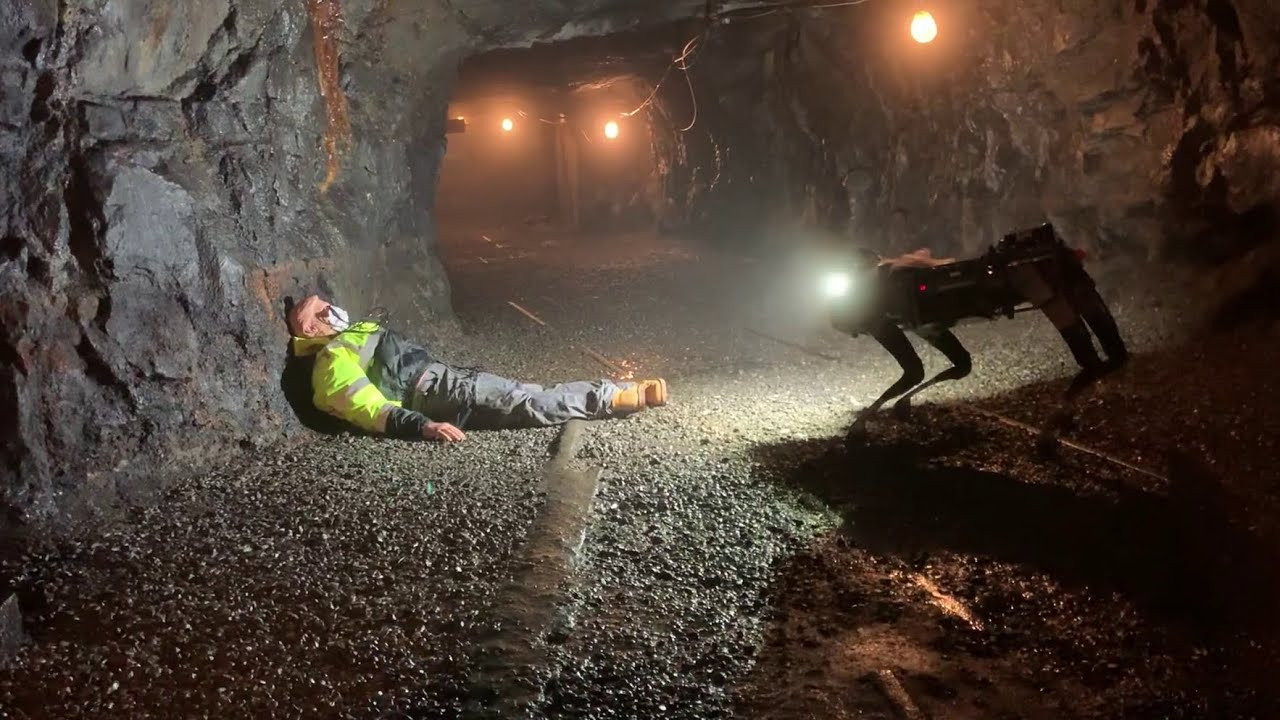
\includegraphics[height=3cm,width=1\textwidth,keepaspectratio]{open_cave.jpg}
                \caption*{DARPA Subterranean Challenge}
                \label{fig:open_cave.jpg}
            \end{figure}
        \end{column}
    \end{columns}
\end{frame}

\begin{frame}[t]{Предментая область: Пещеры}
    \framesubtitle{}
    \vspace{-0.8cm}
    \begin{figure}[H]
        \begin{subfigure}{0.49\textwidth}
            \begin{subfigure}[b]{0.49\textwidth}
                \centering
                \begin{tikzpicture}
                    % Include the image in a node
                    \node [above right, inner sep=0] (image) at (0,0)
                    {\centering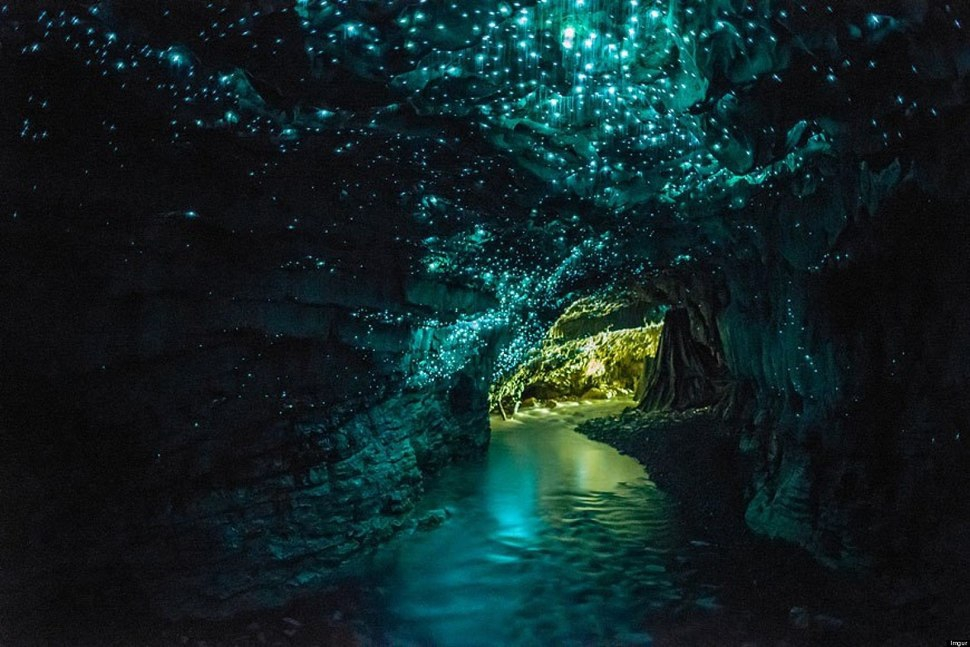
\includegraphics[height=2.5cm,width=1\textwidth,keepaspectratio]{surface_types/splash.png}};
                    % Create scope with normalized axes
                    \begin{scope}[
                            x={($ 0.1*(image.south east)$)},
                            y={($ 0.1*(image.north west)$)}]
                        % Labels
                        \draw[stealth-, very thick,green] (5,2) -- ++(-2,+1)
                        node[rounded corners=3pt,left,black,fill=white]{\tiny Лужа};
                    \end{scope}
                \end{tikzpicture}
                \caption{Лужа}
            \end{subfigure}
            \hfill
            \begin{subfigure}[b]{0.49\textwidth}
                \centering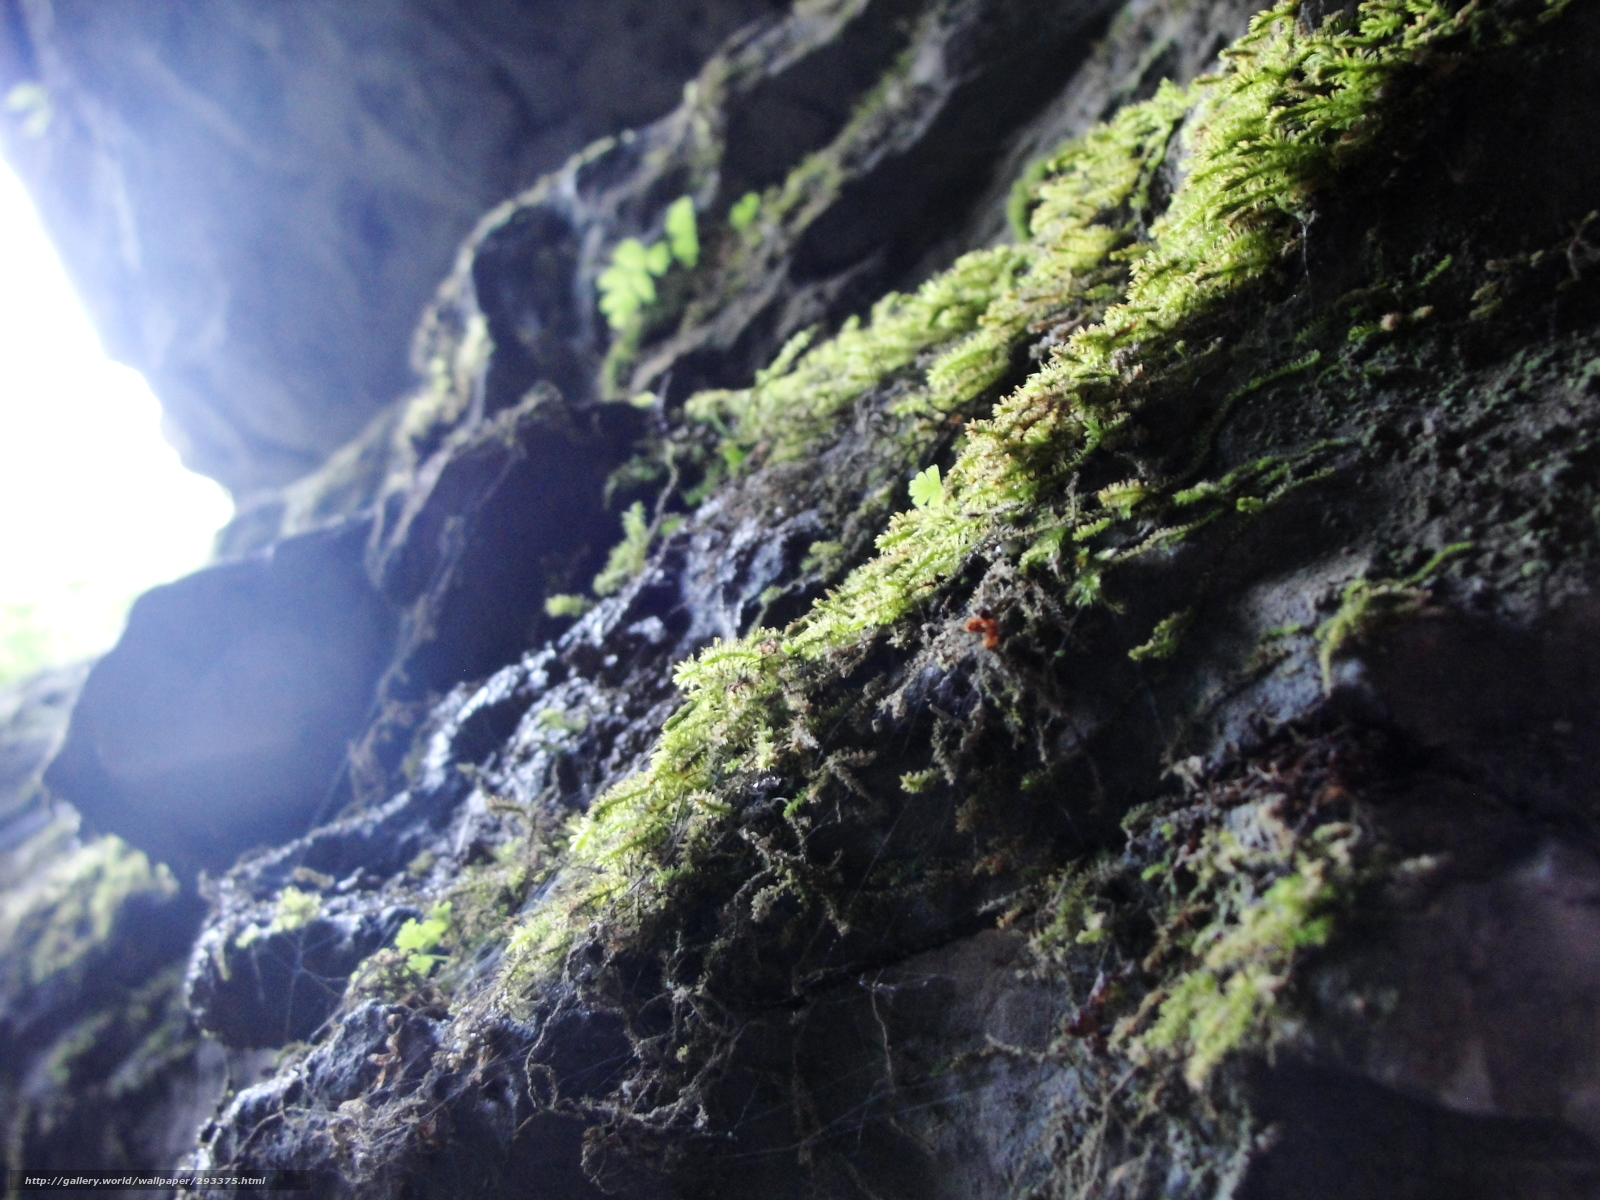
\includegraphics[height=2.5cm,width=1\textwidth,keepaspectratio]{surface_types/moss.jpg}\\
                \caption{Мох}
            \end{subfigure}

            \begin{subfigure}[b]{0.49\textwidth}
                \centering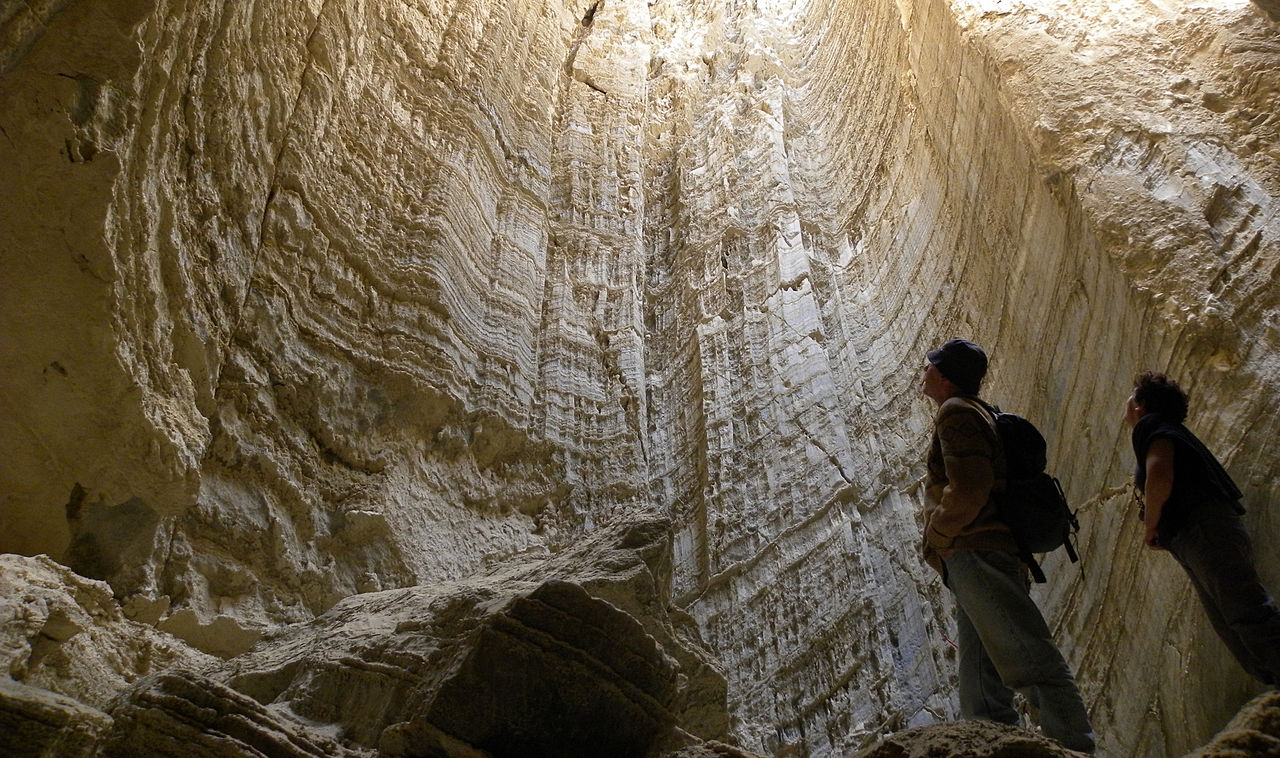
\includegraphics[height=2.5cm,width=1\textwidth,keepaspectratio]{surface_types/salt.jpg}\\
                \caption{Твердые породы}
            \end{subfigure}
            \begin{subfigure}[b]{0.49\textwidth}
                \centering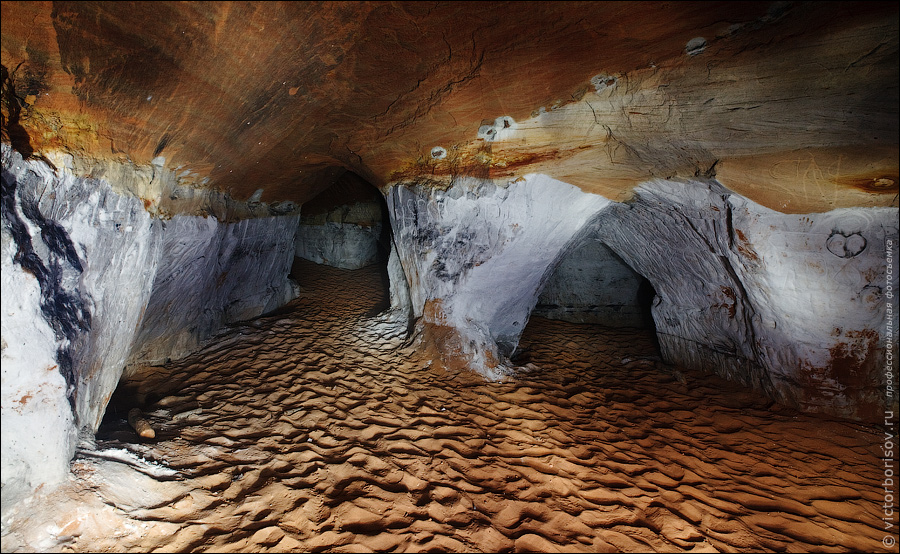
\includegraphics[height=2.5cm,width=1\textwidth,keepaspectratio]{surface_types/sand.jpg}\\
                \caption{Земля}
            \end{subfigure}
            \caption*{Типы опорных поверхностей}
        \end{subfigure}
        \begin{subfigure}{0.49\textwidth}
            \begin{subfigure}{0.99\textwidth}
                \centering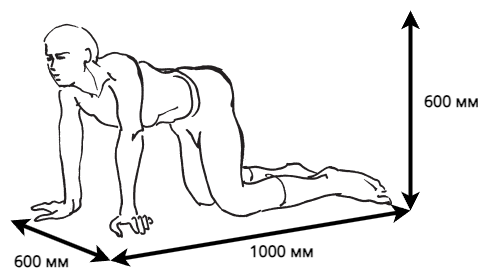
\includegraphics[height=3cm,width=1\textwidth,keepaspectratio]{../images/human_crawling.png}
                \caption*{Габариты пещеры}
            \end{subfigure}

            \begin{subfigure}{0.99\textwidth}
                \centering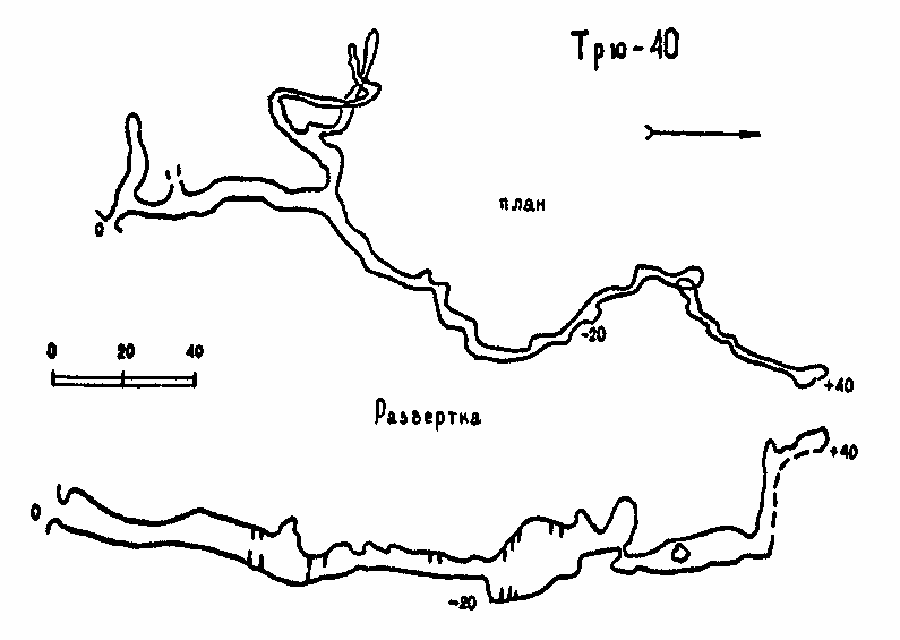
\includegraphics[height=3cm,width=1\textwidth,keepaspectratio]{../images/cave_maps/map3.png}
                \caption*{Протяженность пещер: 1--2 км}
            \end{subfigure}
        \end{subfigure}
    \end{figure}
\end{frame}



\begin{frame}[t]{Вопрос: Как картографировать поверхность под лужей?}
    \framesubtitle{}
    \vspace{-1cm}
    \begin{columns}[T,onlytextwidth]
        \begin{column}{0.44\textwidth}
        \end{column}
        \begin{column}{0.44\textwidth}
            \begin{figure}[H]
                \begin{subfigure}[b]{0.9\textwidth}
                    \centering
                    \begin{tikzpicture}
                        % Include the image in a node
                        \node [above right, inner sep=0] (image) at (0,0)
                        {\centering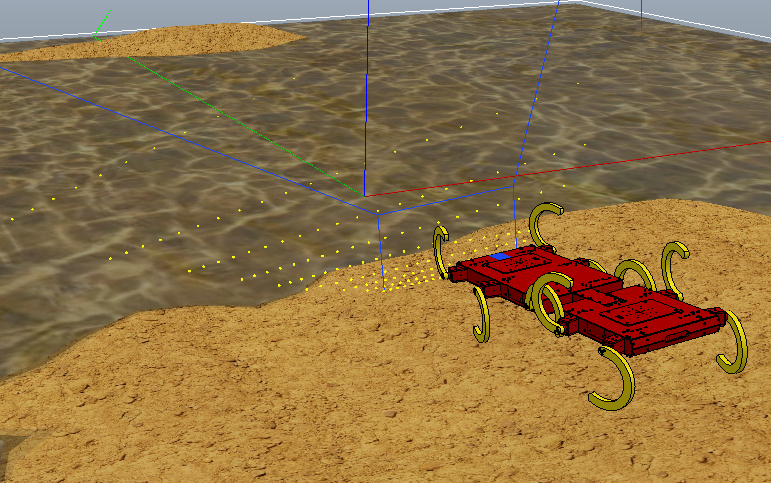
\includegraphics[height=3.5cm,width=1\textwidth,keepaspectratio]{terrain_w_water1.png}};
                        % Create scope with normalized axes
                        \begin{scope}[
                                x={($ 0.1*(image.south east)$)},
                                y={($ 0.1*(image.north west)$)}]
                            \draw[stealth-, very thick,green] (6,8) -- ++(2,1)
                            node[rounded corners=3pt,right,black,fill=white]{\tiny Вода};

                            \draw[stealth-, very thick,green] (0.5,5.5) -- (3,2);
                            \draw[stealth-, very thick,green] (2.5,4.2) -- (3,2);
                            \draw[stealth-, very thick,green] (4.5,4) -- (3,2)
                            node[rounded corners=3pt,below,black,fill=white]{\tiny Лазер Лидара};
                        \end{scope}
                    \end{tikzpicture}
                    % \caption*{}
                    \label{fig:terrain_w_water1.png}
                \end{subfigure}
                \vspace{-0.5cm}

                \begin{subfigure}{0.8\textwidth}
                    \centering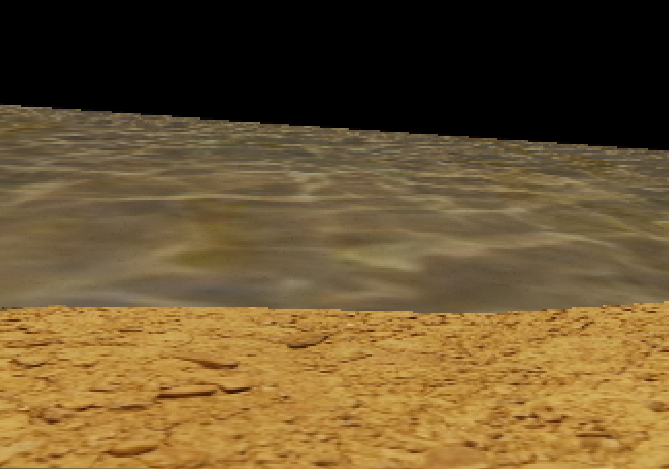
\includegraphics[height=2cm,width=1\textwidth,keepaspectratio]{terrain_w_water_camera.png}
                    \caption*{Вид с камеры}
                \end{subfigure}
            \end{figure}
        \end{column}
    \end{columns}
\end{frame}

\begin{frame}[t]{Цель работы}
    \framesubtitle{}
    Разработать \textbf{метод построения карты местности} с определением \underline{геометрических} и \underline{физико-механических} свойств \textit{опорной поверхности} роботом с шагающими движителями снабженными \underline{тактильными датчиками}, \textit{без использования оптических сенсоров}.
    \begin{figure}[H]
        \begin{subfigure}{0.49\textwidth}
            \centering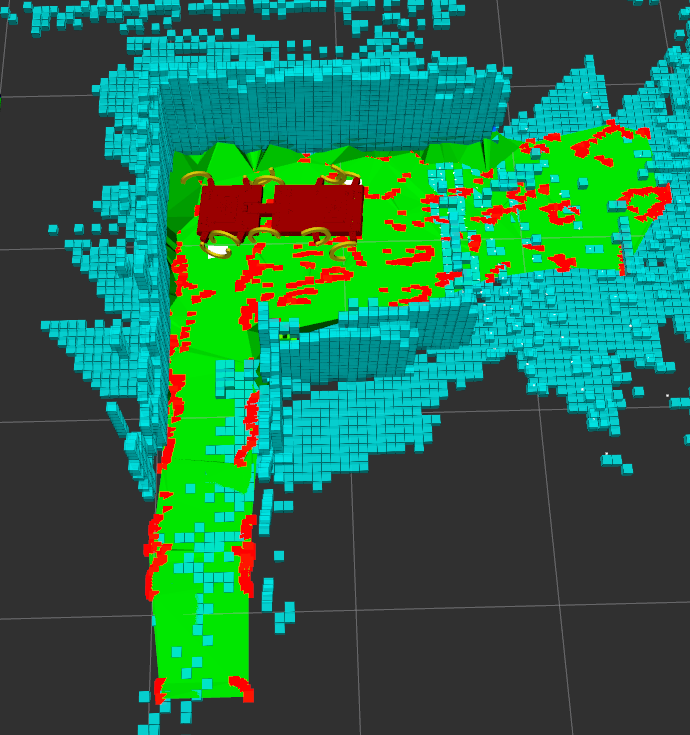
\includegraphics[height=3.5cm,width=1\textwidth,keepaspectratio]{conv_concave.png}
            \caption*{Определение геометрических свойств}
        \end{subfigure}
        \begin{subfigure}{0.49\textwidth}
            \centering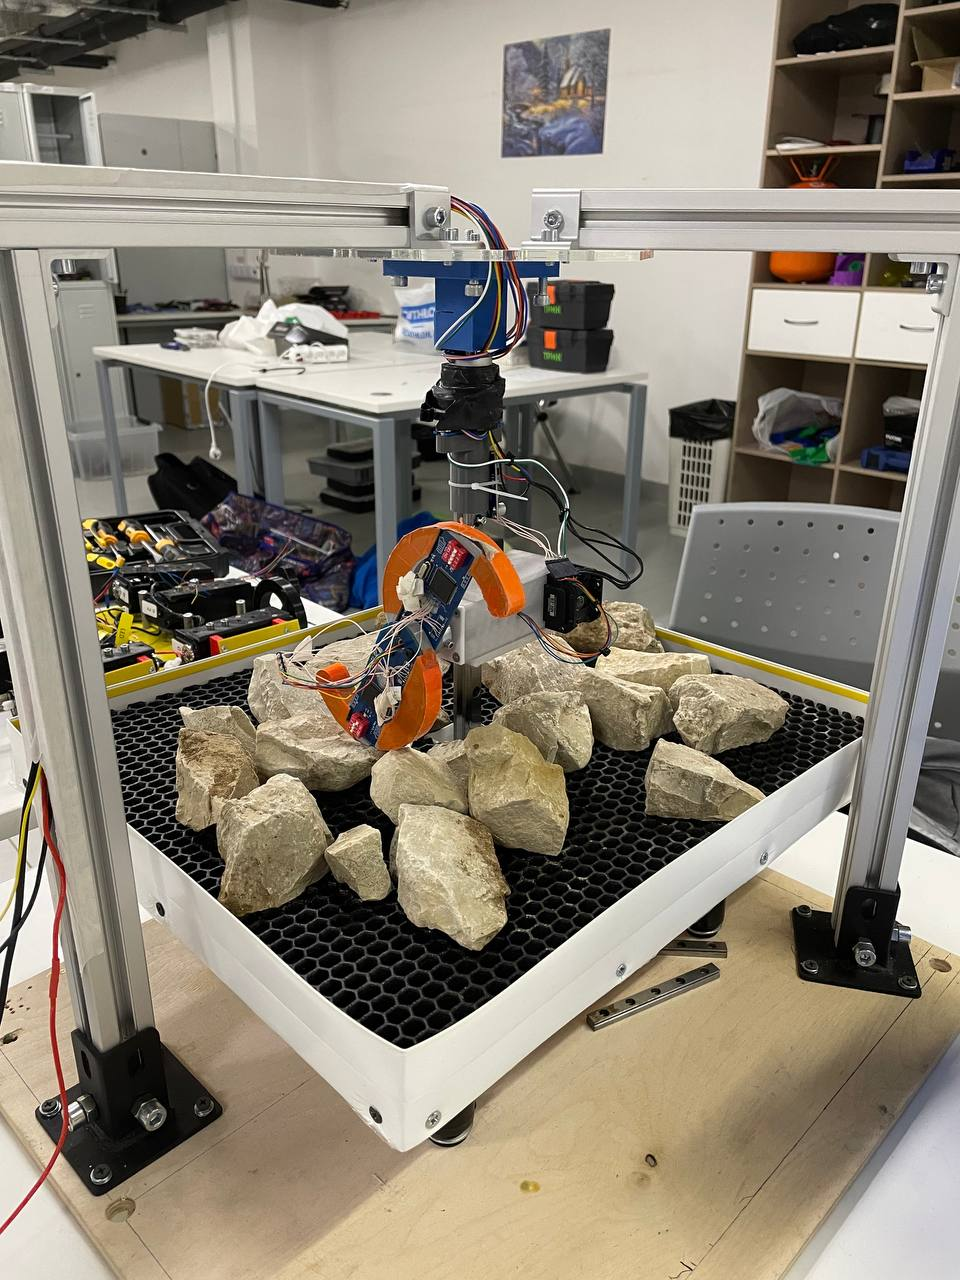
\includegraphics[height=3.5cm,width=1\textwidth,keepaspectratio]{s_shape_leg/view.jpg}
            \caption*{Определение физических свойств}
            \label{fig:s_shape_leg/view.jpg}
        \end{subfigure}
    \end{figure}
\end{frame}

\begin{frame}[t]{"1, 2" Построение рельефа местности}
    \framesubtitle{}
    \begin{columns}[T,onlytextwidth]
        \begin{column}{0.49\textwidth}
            \textbf{Геометрические свойства:}\\
            \textit{Входные данные}: следовая дорожка, представленная в виде облака точек.

            \textit{Выходные данные}: полигональная сетка и плотное облако точек.

            \textit{Допустимая точность}: 0.1 м
            \begin{figure}[H]
                \begin{subfigure}{0.49\textwidth}
                    \centering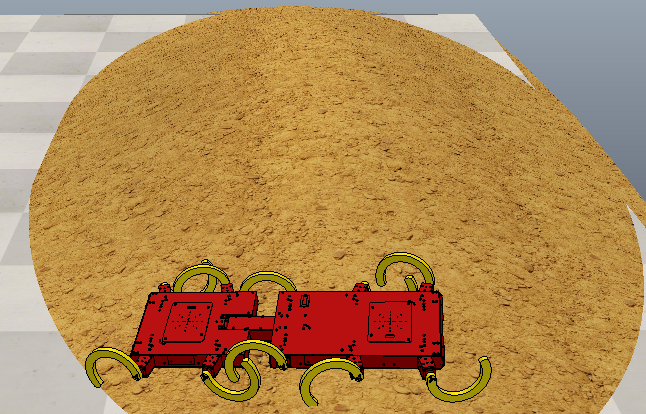
\includegraphics[height=2cm,width=1\textwidth,keepaspectratio]{../images/slides/surface_research.png}
                    \caption{Исследуемая поверхность}
                    \label{fig:../images/slides/surface_research.png}
                \end{subfigure}
                \begin{subfigure}{0.49\textwidth}
                    \centering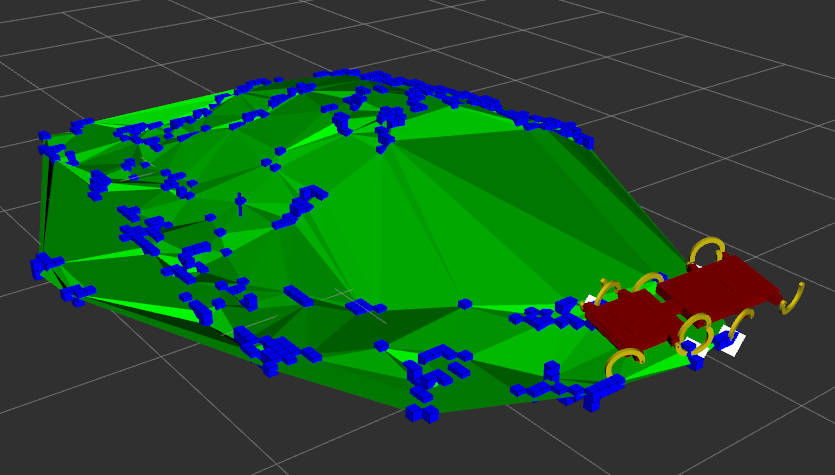
\includegraphics[height=2cm,width=1\textwidth,keepaspectratio]{../images/slides/result_research.png}
                    \caption{Следовая дорожка и полигональная сетка}
                    \label{fig:../images/slides/result_research.png}
                \end{subfigure}
            \end{figure}
        \end{column}
        \begin{column}{0.49\textwidth}
            \textbf{Физико-механические свойства:}\\
            \textit{Входные данные}: обученный классификатор поверхностей, данные с внутренних датчиков робота.

            \textit{Выходные данные}: процентное соотношение упругих, твердых и пластичных свойств пройденной поверхности.

            \textit{Допустимая ошибка}: 20% 

            \begin{figure}[H]
                \begin{subfigure}{0.49\textwidth}
                    \centering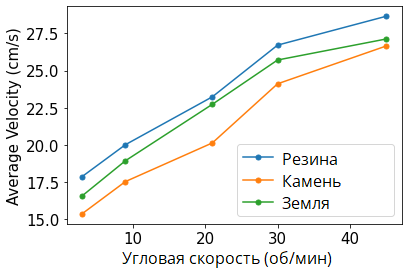
\includegraphics[height=2cm,width=1\textwidth,keepaspectratio]{../images/slides/avg_lin_vel_rev_min.png}
                    \caption{График зависимости угловой скорости мотора от линейного перемещения робота по различным поверхностям}
                    \label{fig:../images/slides/avg_lin_vel_rev_min.png}
                \end{subfigure}
                \begin{subfigure}{0.49\textwidth}
                    \centering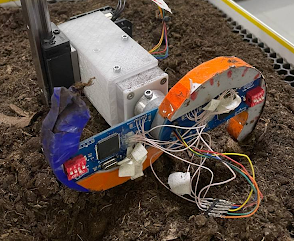
\includegraphics[height=2cm,width=1\textwidth,keepaspectratio]{../images/slides/data.png}
                    \caption{Пример поверхности}
                    \label{fig:../images/slides/data.png}
                \end{subfigure}
            \end{figure}
        \end{column}
    \end{columns}
\end{frame}


\begin{frame}[t]{Объект исследования}
    \framesubtitle{}
    \begin{columns}[T,onlytextwidth]
        \begin{column}{0.54\textwidth}
            \textbf{Класс многоногих шагающих роботов} с цельным или сочленённым корпусом, и цикловыми движителями с одной степенью свободы, управляемые зависимо или независимо друг от друга.

            \textit{Требования к данному классу}:
            \begin{itemize}
                \item Компактные размеры (меньше чем $1000\times600\times600$ мм)
                \item Залезать на препятствия высотой меньше, чем $\frac{3}{4}$ длины корпуса
                \item Преодолевать представленные
                      опорные поверхности
            \end{itemize}
        \end{column}
        \begin{column}{0.44\textwidth}
            \begin{figure}[H]
                \hfill
                \begin{subfigure}{0.99\textwidth}
                    \centering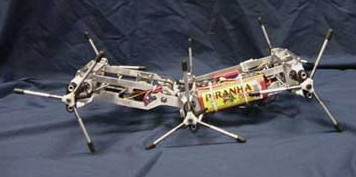
\includegraphics[height=2cm,width=1\textwidth,keepaspectratio]{from_master/whegs2.jpg}
                    \caption{WHegs}
                    \label{fig:from_master/whegs2.jpg}
                \end{subfigure}

                \hfill
                \begin{subfigure}{0.49\textwidth}
                    \centering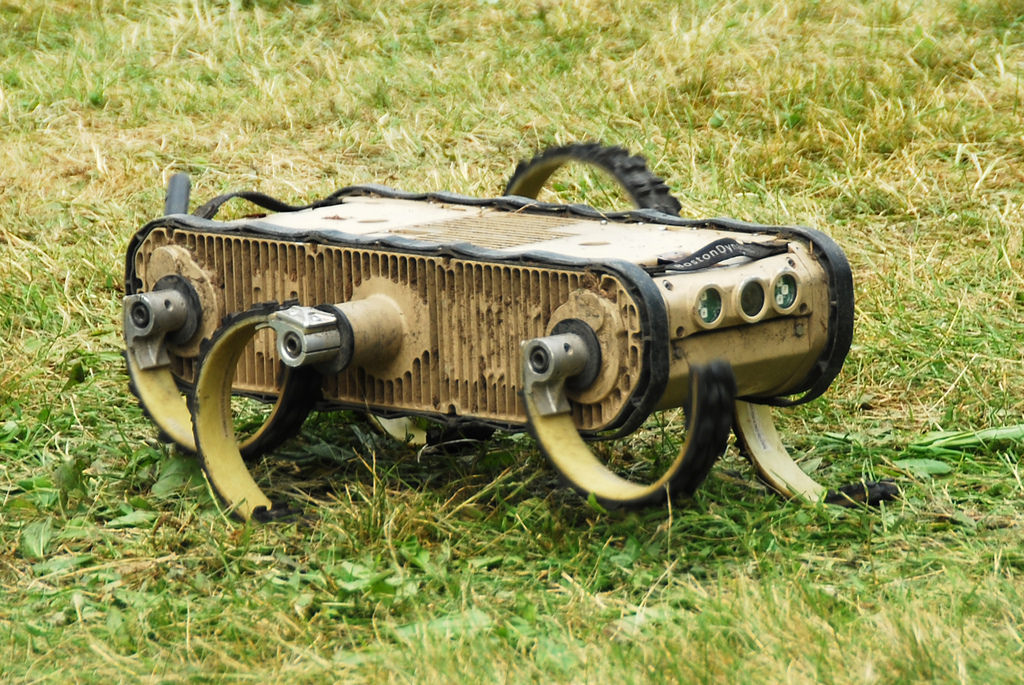
\includegraphics[height=2cm,width=1\textwidth,keepaspectratio]{from_master/rhex.jpg}
                    \caption{Boston Dynamics RHex}
                    \label{fig:from_master/rhex.jpg}
                \end{subfigure}
                \begin{subfigure}{0.49\textwidth}
                    \centering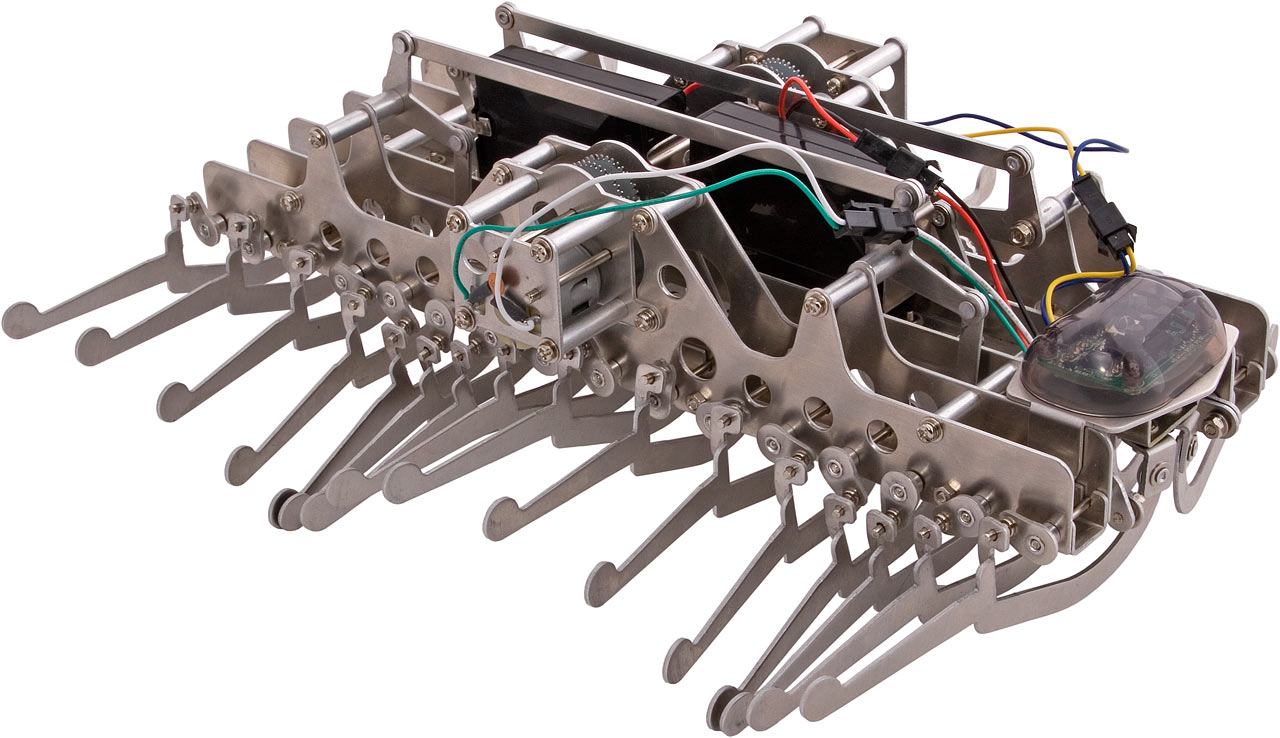
\includegraphics[height=2cm,width=1\textwidth,keepaspectratio]{from_master/gakken.jpg}
                    \caption{Gakken Centipede}
                    \label{fig:from_master/gakken.jpg}
                \end{subfigure}
            \end{figure}
        \end{column}
    \end{columns}
\end{frame}

\begin{frame}[t]{"3" Оптимизация кинематической схемы}
    \framesubtitle{}
    \begin{columns}[T,onlytextwidth]
        \begin{column}{0.49\textwidth}
            Решить $F=f(x) \rightarrow max$ критерий оптимизации, где

            $f(x)$ --- критерии: пройденная дистанция, длина корпуса\\
            $(x)$ --- параметр: количество ног

            \textit{Количество ног имеет прямую зависимость с длиной корпуса робота.}
        \end{column}
        \begin{column}{0.49\textwidth}
            \vspace{-0.5cm}
            \begin{figure}[H]
                \begin{subfigure}{0.99\textwidth}
                    \centering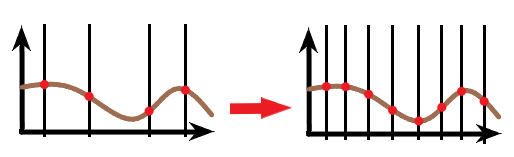
\includegraphics[height=1.8cm,width=1\textwidth,keepaspectratio]{f1.png}
                    \caption*{Кол-во ног $\uparrow$, детализация поверхности $\downarrow$}
                    \label{fig:f1.png}
                \end{subfigure}

                \begin{subfigure}{0.99\textwidth}
                    \centering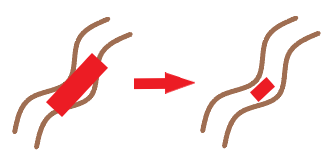
\includegraphics[height=1.8cm,width=1\textwidth,keepaspectratio]{f2.png}
                    \caption*{Длина робота $\uparrow$, курсовая проходимость $\downarrow$}
                    \label{fig:f2.png}
                \end{subfigure}

                \begin{subfigure}{0.99\textwidth}
                    \centering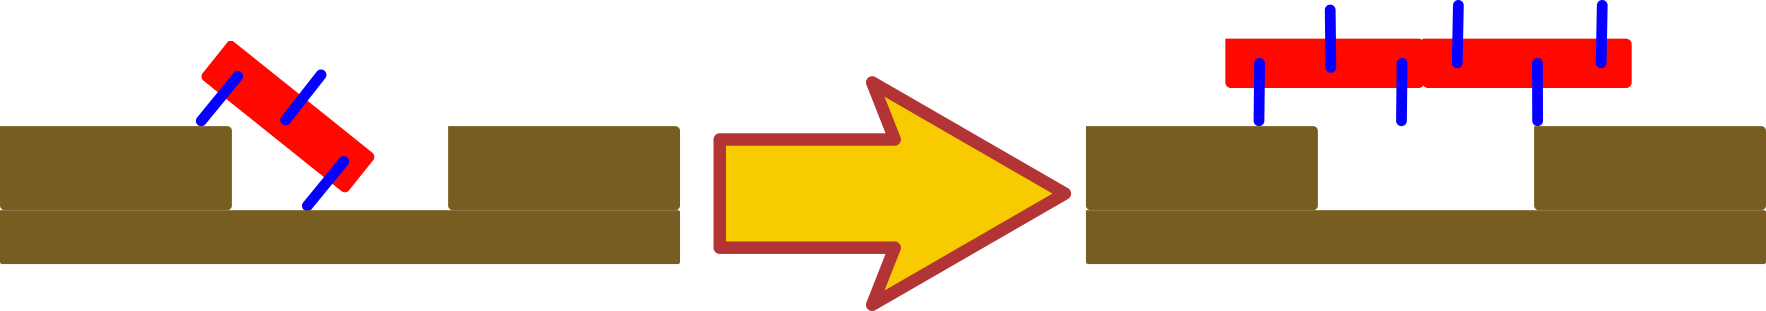
\includegraphics[height=1.8cm,width=1\textwidth,keepaspectratio]{f3_new.png}
                    \caption*{Длина робота $\uparrow$, проходимость $\uparrow$}
                    \label{fig:f3.png}
                \end{subfigure}
            \end{figure}
        \end{column}
    \end{columns}
\end{frame}

\begin{frame}[t]{"4" Верификация преобразователя силы}
    \framesubtitle{}
    \begin{columns}[T,onlytextwidth]
        \begin{column}{0.49\textwidth}
            Охарактеризовать материал для случаев, когда площадь приложения силы меньше, чем площадь активной части сенсора.

            \textit{Входные данные}: показания разработанного датчика и значение реально приложенной нагрузки

            \textit{Выходные данные}: разница между нормализованным значением с датчика и реальной нагрузкой

            \textit{Допустимая ошибка}: 10% 
        \end{column}
        \begin{column}{0.49\textwidth}
            \begin{figure}[H]
                \begin{subfigure}{0.9\textwidth}
                    \centering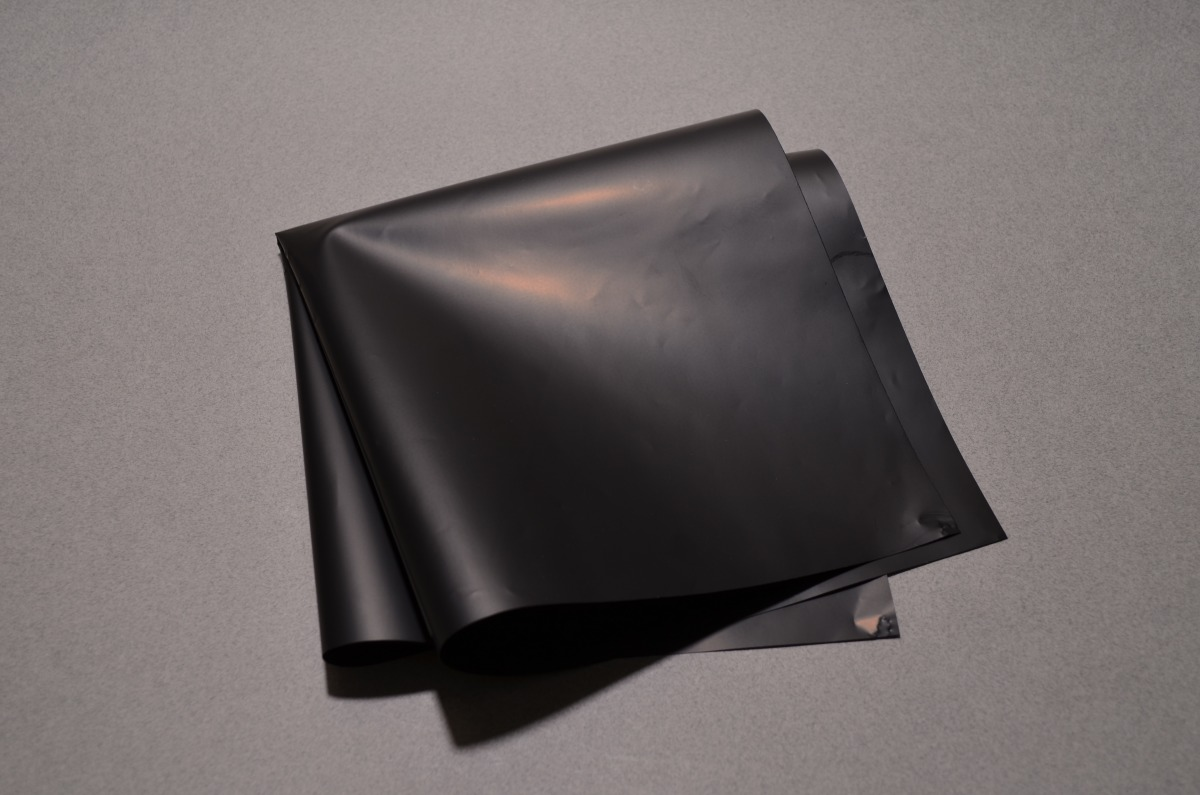
\includegraphics[height=2cm,width=1\textwidth,keepaspectratio]{velostat_sensor.jpg}
                    \caption{Материал Velostat}
                    \label{fig:velostat_sensor.jpg}
                \end{subfigure}

                \begin{subfigure}{0.9\textwidth}
                    \centering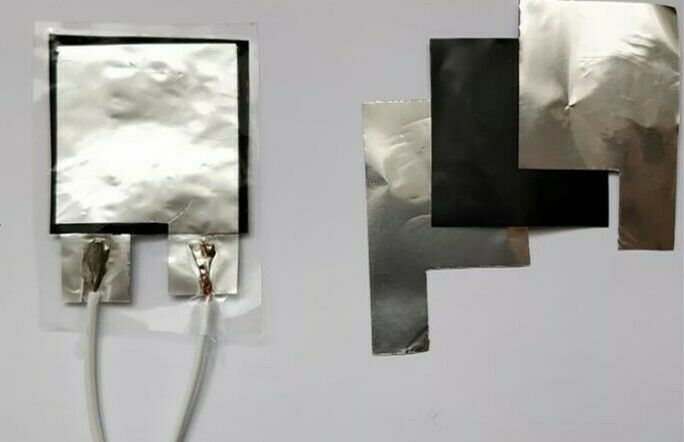
\includegraphics[height=2cm,width=1\textwidth,keepaspectratio]{simplest_sensor.jpg}
                    \caption{Простейший преобразователь силы}
                    \label{fig:simplest_sensor.jpg}
                \end{subfigure}
            \end{figure}
        \end{column}
    \end{columns}
\end{frame}

\begin{frame}[t]{Структура}
    \framesubtitle{}
    \begin{figure}[H]
        \centering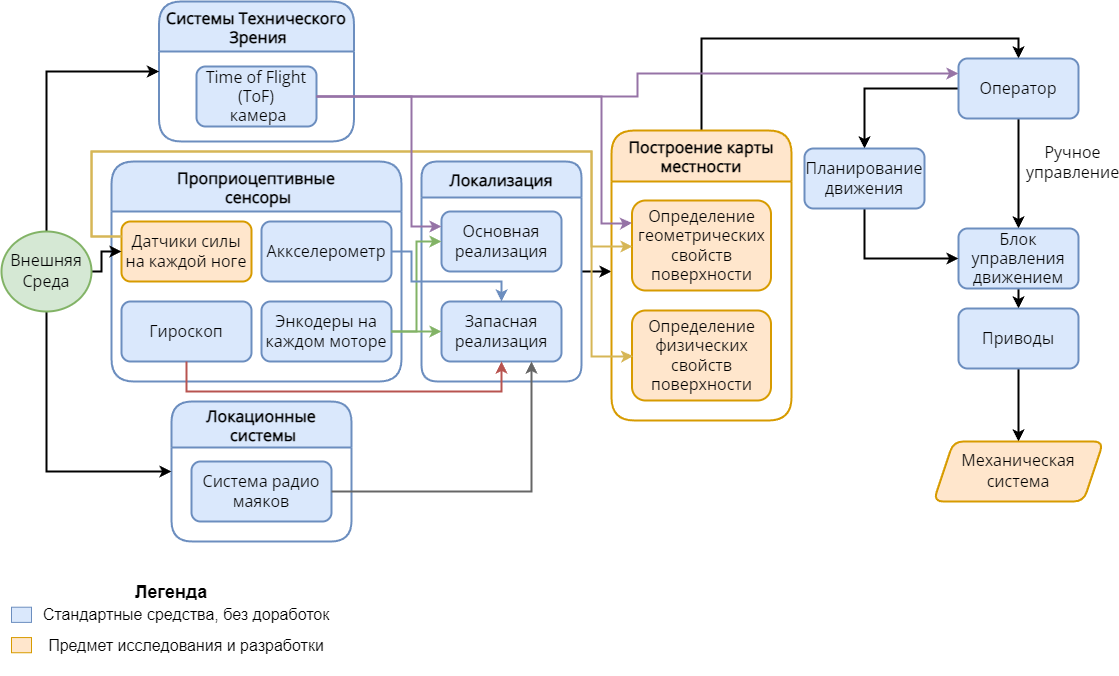
\includegraphics[height=6.5cm,width=1\textwidth,keepaspectratio]{main_diag_hor.png}
        \label{fig:main_diag_hor.png}
    \end{figure}
\end{frame}

\begin{frame}[t]{Основные научные задачи исследования}
    \framesubtitle{}
    \begin{enumerate}
        \item  Разработка метода \textbf{построения карты местности и определения геометрических свойств поверхности} с помощью тактильного очувствления.
        \item Реализация алгоритма, позволяющего \textbf{определять физические свойства} опорной поверхности.
        \item Разработка метода \textbf{оптимизации конструкции многоногих шагающих роботов} с цикловыми движителями с одной степенью свободы критериям проходимости, покрытия опорной поверхности и её детализации, длины пройденного пути.
        \item Создание методики \textbf{исследования датчика силы}, когда площадь контакта нажатия на сенсор меньше чувствительной области самого сенсора.
    \end{enumerate}
\end{frame}

\begin{frame}{Положения, выносимые на защиту}
    \begin{enumerate}
        \vspace{-0.3cm}
        \small
        \item \textbf{Метод построения карты местности}, состоящий в определении геометрической формы поверхности с помощью тактильного очувствления, который позволяет решать задачу определения плана и профиля поверхности в условиях отсутствия видимости и при движении по поверхности, находящейся под водой.
        \item \textbf{Метод определения физико-механических свойств опорной поверхности} на основе \textbf{тактильного очувствления}, позволяющий различать материалы с \textit{упругими, жёсткими, пластичными свойствами}.
        \item \textbf{Критерий оптимизации} кинематической схемы многоногих шагающих роботов с цикловыми одностепенными движителями, включающий в себя показатели проходимости, покрытия опорной поверхности и её детализации. Определение на его основе габаритов и количества движителей шагающего робота.
        \item \textbf{Зависимость} \textit{погрешности} датчика силы на основе полимерного материла от \textit{площади пятна контакта} относительно размеров датчика, применяемого для тактильного очувствления мобильного робота. \textbf{Методика} роботизированного исследования датчика силы.
    \end{enumerate}
\end{frame}

\section{Обзор существующих решений}

\begin{frame}[t]{Литературный обзор}
    \framesubtitle{}
    \begin{itemize}
        \item \textbf{Задача оптимизации конструкции}: Б. Петриашвили (СССР), Stefano Nolfi (Италия), Dario Sanch-Pradel (Италия), S. Feng (США)
        \item \textbf{Шагающие цикловые роботы}: Е. С. Брискин (Россия), Ю. Д. Андриантов (СССР), Edward Z. Moore (Канада), Wei-Hsi Chen (Китай)
        \item \textbf{Верификация Velostat}:  Igor Vehec (Словакия),  Robert Schroer (США)
        \item \textbf{Определение геометрических свойств поверхности}: Tobias Ebert (Германия), Subodh Kumar (США), И. Рядчиков (Россия), Shan Luo (Британия)
        \item \textbf{Определение физико-механических свойств поверхности}: X. Alice Wu (США), Krzysztof Walas (Польша), Hendrik Kolvenbach (Швейцария)
    \end{itemize}
\end{frame}

\section{"3" Оптимизация кинематической схемы}

\begin{frame}[t]{Определение количества ног}
    \framesubtitle{}
    \begin{columns}[T,onlytextwidth]
        \begin{column}{0.59\textwidth}
            \small
            Решить $F=f(x) \rightarrow max$ критерий оптимизации, где

            $f(x)$ --- \textbf{ Критерии}: пройденная дистанция, длина корпуса\\
            $(x)$ --- \textbf{Параметры}: количество ног, сдвиг фазы между
            соседними ногами

            \textbf{Метод решения}: Генетический алгоритм: Open AI-ES

            \textbf{Идея решения}: генерируется множество особей, а
            также семейство территорий с одинаковой сложностью.
            За фиксированное время, с постоянной угловой скоростью
            на моторах, каждый робот проходит это семейство
            территорий и записываются данные.

            \textbf{Предположения}: 1) есть только сухое трение
            между ногами и поверхностью. 2) Созданные
            поверхности с помощью одной функции
            и параметров имеют одинаковую сложность.

            \textbf{Утверждение}:\textit{Количество ног имеет прямую
                зависимость с длиной корпуса робота.}
        \end{column}
        \begin{column}{0.39\textwidth}
            \begin{figure}[H]
                \begin{subfigure}{0.49\textwidth}
                    \centering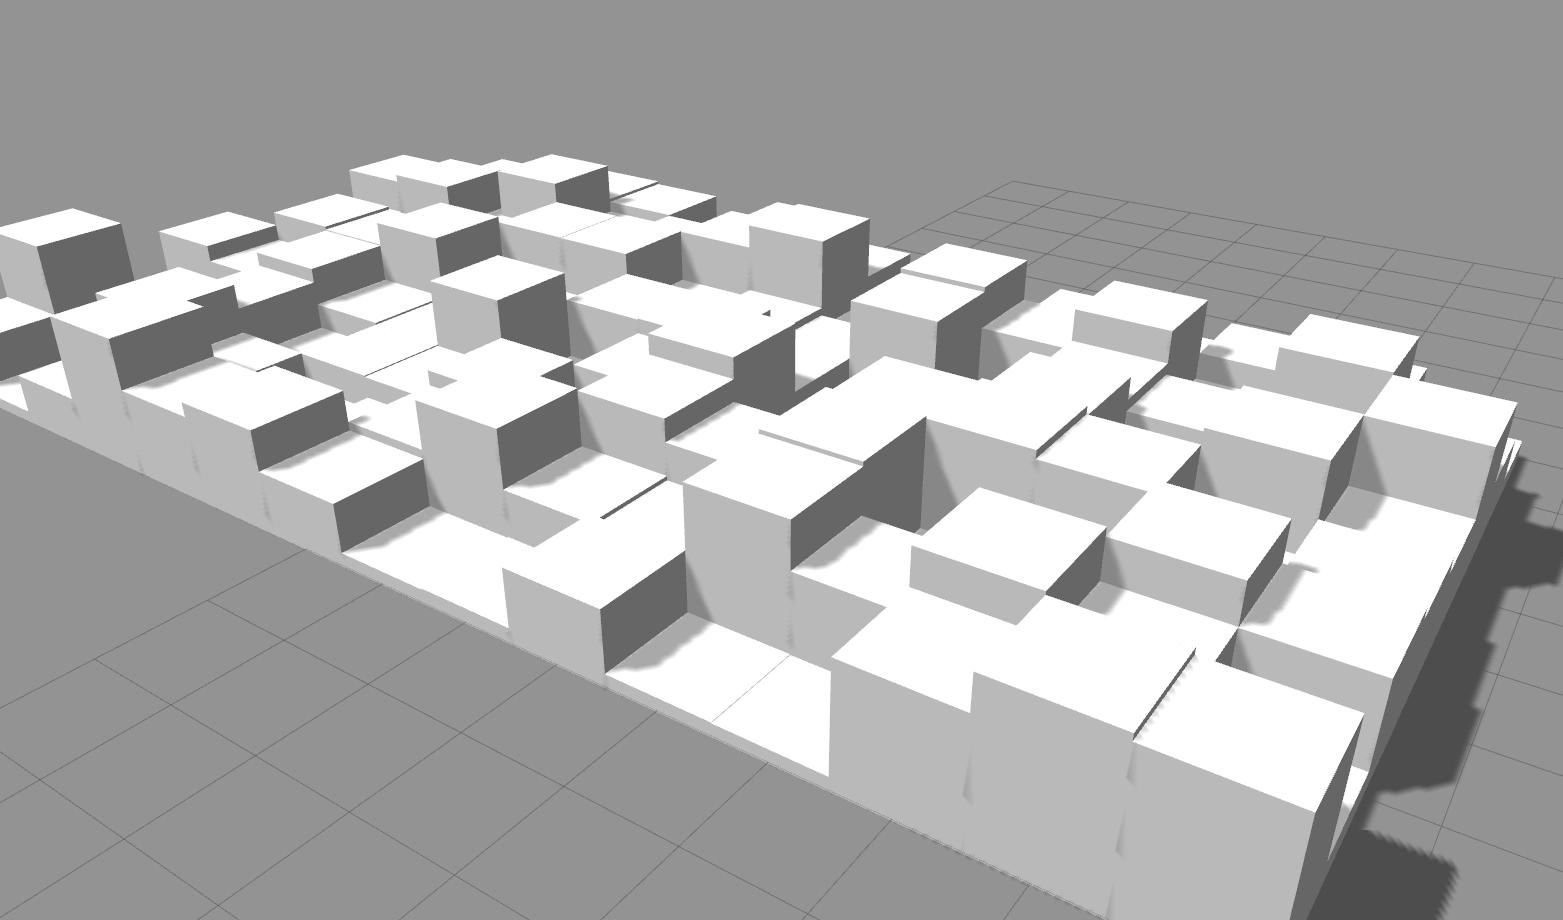
\includegraphics[height=2cm,width=1\textwidth,keepaspectratio]{../images/terrain_1.jpg}
                    % \caption{capture1}
                \end{subfigure}
                \begin{subfigure}{0.49\textwidth}
                    \centering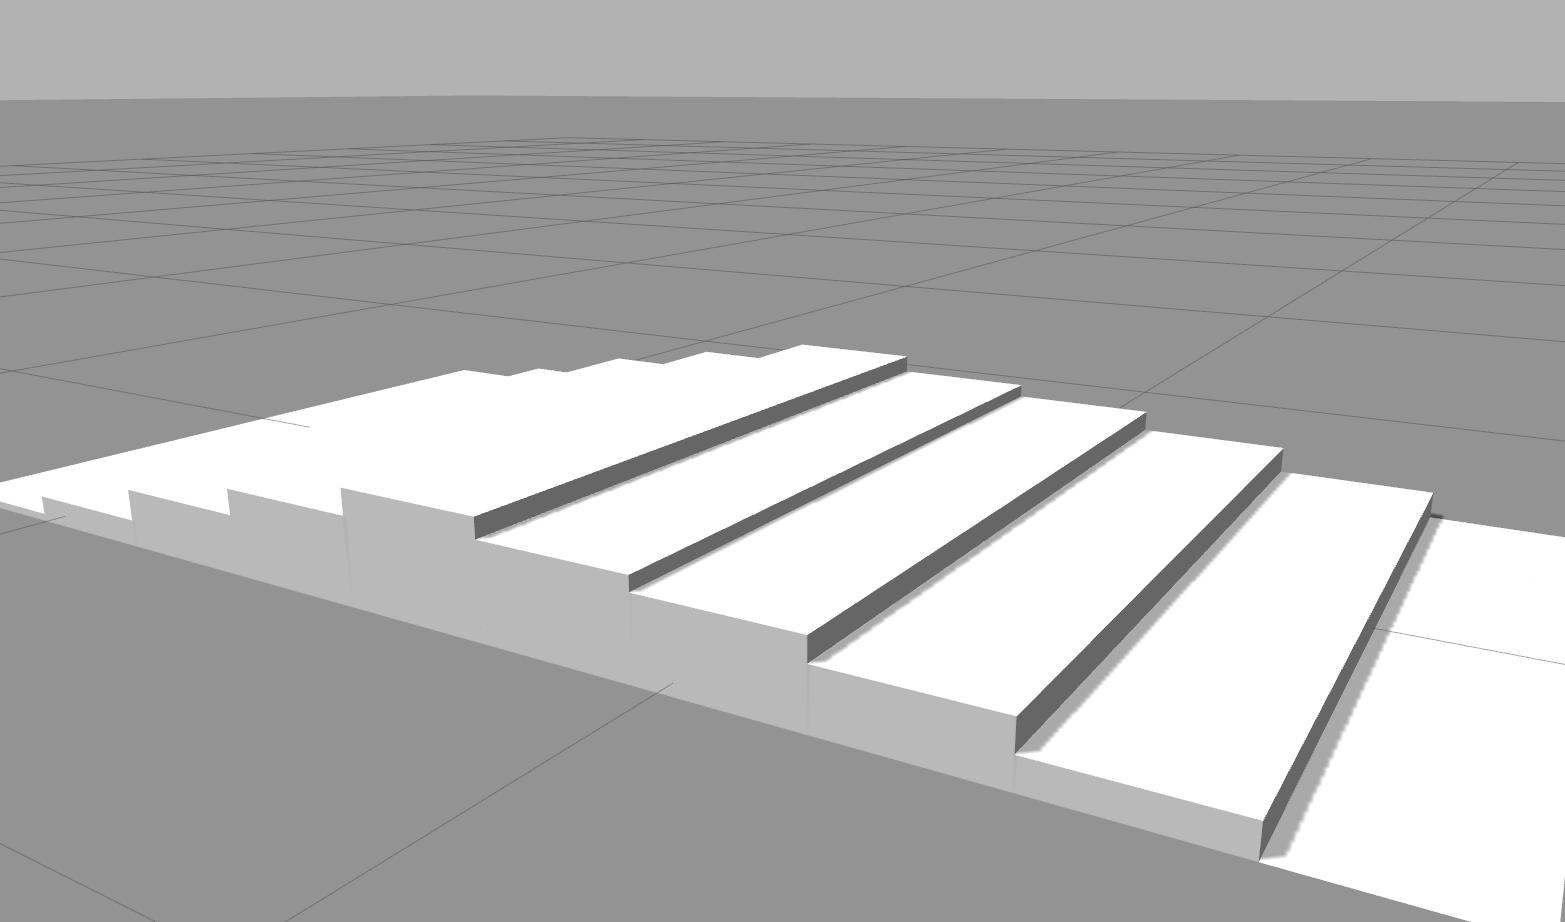
\includegraphics[height=2cm,width=1\textwidth,keepaspectratio]{../images/terrain_2.jpg}
                    % \caption{capture2}
                \end{subfigure}

                \begin{subfigure}{0.99\textwidth}
                    \centering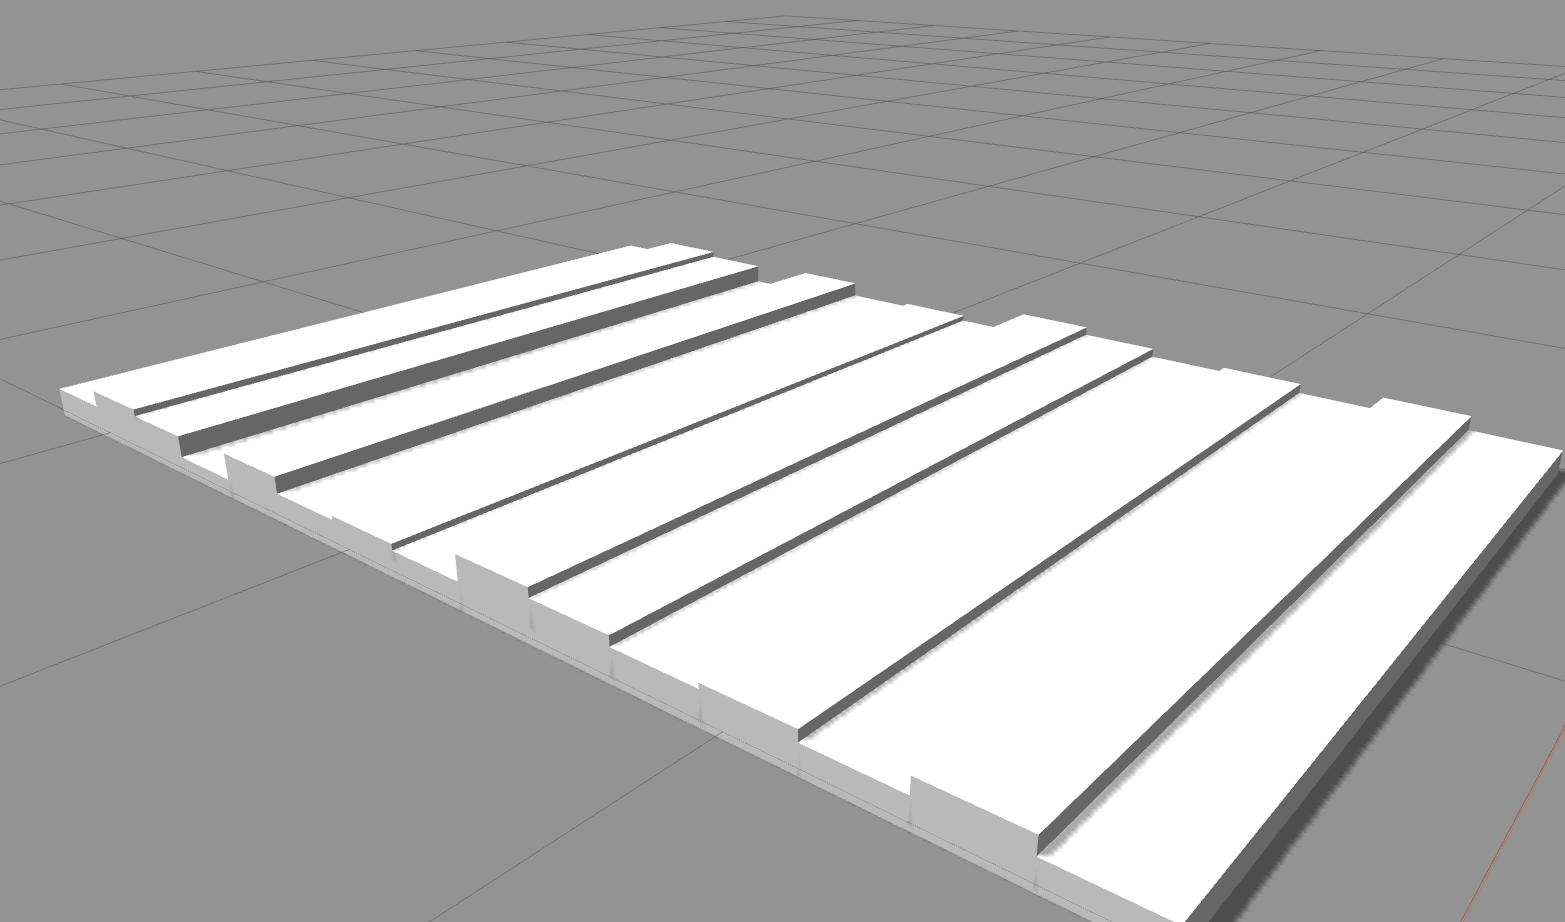
\includegraphics[height=2.5cm,width=1\textwidth,keepaspectratio]{../images/terrain_3.jpg}
                    \caption*{Пример прохождения особью сгенерированной поверхности}
                    \label{fig:../images/terrain_3.jpg}
                \end{subfigure}
            \end{figure}
        \end{column}
    \end{columns}
\end{frame}

\begin{frame}[t]{Целевая функция}
    \framesubtitle{}
    \vspace{-0.4cm}
    \begin{columns}[T,onlytextwidth]
        \begin{column}{0.48\textwidth}
            \begin{eqnarray}
                F \rightarrow max = \beta \left( {\omega}_{1} \cdot \delta + {\omega}_{2} \cdot L\right) + \\ \nonumber + (1 - \beta) {\delta}^{{\omega}_{1}} {\left( L\right)}^{{\omega}_{2}} \\
                L = \frac{1}{(\gamma - 1) h_{\text{leg}}sin(\alpha)}
            \end{eqnarray}
            Где
            $\beta$ -- адаптивный параметр, \\ ${\omega}_{1,2} \in  [ 0..1 ] $ -- весовые коэффициенты, \\
            $\delta$ -- пройденный путь, \\
            $L$ -- упрощенная длина робота

            \textit{Для решения однокритериальной задачи} использовалась аддитивно-мультипликативная свертка
        \end{column}
        \begin{column}{0.50\textwidth}
            \begin{figure}[H]
                \centering
                \begin{tikzpicture}
                    % Include the image in a node
                    \node [above right, inner sep=0] (image) at (0,0)
                    {\centering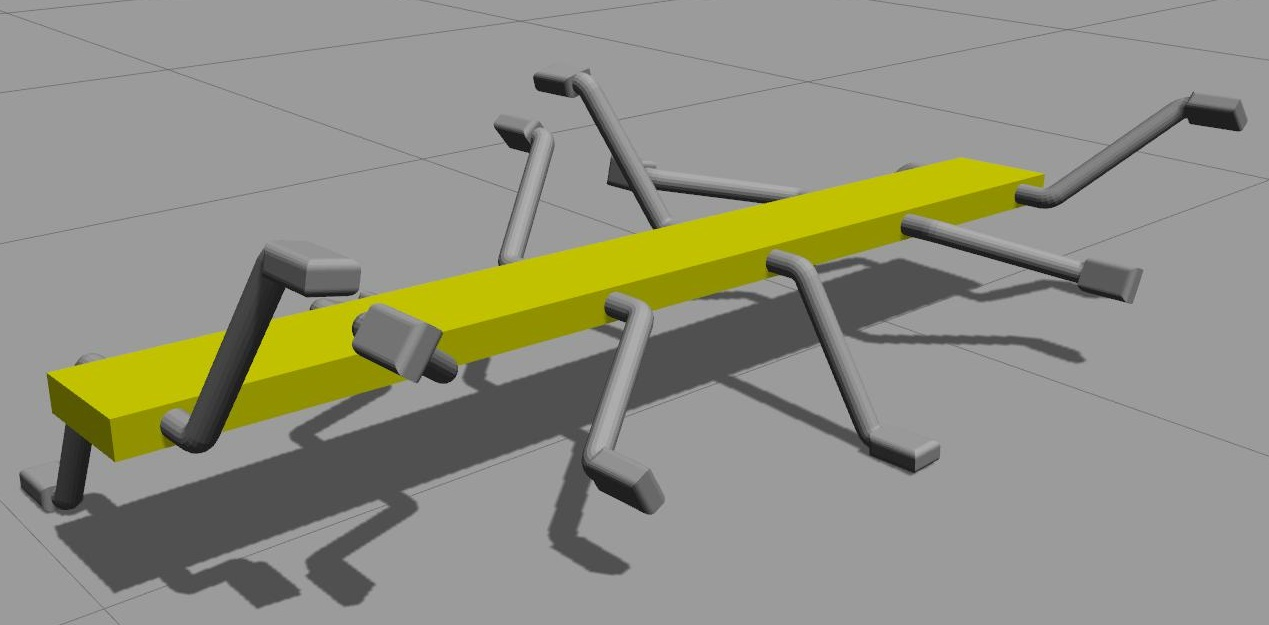
\includegraphics[height=3cm,width=1\textwidth,keepaspectratio]{best_gen_robot.jpg}};
                    % Create scope with normalized axes
                    \begin{scope}[
                            x={($ 0.1*(image.south east)$)},
                            y={($ 0.1*(image.north west)$)}]
                        % Labels
                        \draw [green, very thick,
                            decorate,
                            decoration = {brace,
                                    raise=5pt,
                                    amplitude=5pt,
                                    aspect=0.5}] (1.4,3.6) --  (8.1,6.8)
                        node[rounded corners=3pt, pos=0.5,above left =14pt,black,fill=white]{\tiny $(\gamma - 1) h_{\text{leg}}sin(\alpha)$};

                        \draw[stealth-, very thick,green] (9.5,7.8) -- (7.8,1.94);
                        \draw[stealth-, very thick,green] (1.5,2.8) -- (7,1)
                        node[rounded corners=3pt,right,black,fill=white]{\tiny $\gamma = 6$};

                        \draw[thin,green] (6.7,4) -- (5.75,9);
                        \draw[thin,green] (4.85,3.5) -- (5.75,9);
                        \draw[thin,green,stealth-stealth] (6.32,6) arc (-79.2:-99.2:3) node [rounded corners=3pt,below = 2pt,black,fill=white, midway] {\tiny $\alpha$};
                    \end{scope}
                \end{tikzpicture}
            \end{figure}
        \end{column}
    \end{columns}
\end{frame}

\begin{frame}[t]{Описание механической системы}
    \framesubtitle{}
    \begin{align}
        M \dot{\vec{u}} = \vec{g}                                \\
        M = \begin{bmatrix}
                M_1    & \cdots & 0      \\
                \vdots & \ddots & \vdots \\
                0      & \cdots & M_n
            \end{bmatrix},\ M_i = \begin{bmatrix}
                                      m_i E_{3\times 3} & 0   \\
                                      0                 & I_i
                                  \end{bmatrix}        \\
        \vec{u}_i^{\ T} = \begin{bmatrix}
                              \vec{v}_i^{\ T} & \vec{\omega}_i^{\ T}
                          \end{bmatrix} \\
        \vec{g}^{\ T} = \begin{bmatrix}
                            \cdots \  \vec{F}_i^{\ T}, & (\vec{\tau}_i - \vec{\omega}_i \times I_i \vec{\omega}_i)^T\  \cdots
                        \end{bmatrix}
    \end{align}
    где, $M_i$~---~матрицы, содержащие массово-инерционные характеристики; $m_i$~---~масса тела; $I_i$~---~тензор инерции; $\vec{u_i}$~---~вектор обобщённых скоростей; $E$~---~единичная матрица; $\vec{g}$~---~вектор обобщённых сил; $\vec{v_i}$~---~вектор линейной скорости; $\vec{\omega_i}$~---~вектор угловой скорости; $\vec{F_i}$, $\vec{\tau_i}$~---~силы и моменты сил взаимодействия.
\end{frame}

\begin{frame}[t]{Геометрические связи}
    \framesubtitle{}
    Тела соединены цилиндрическими шарнирами:
    \begin{align}
        \phi(q_{j_1},\ u_{j_1},\ \cdots,\ q_{j_k},\ u_{j_k},\ t) \geqslant  0 \\
        \vec{q_i}^{\ T} = \begin{bmatrix}
                              \vec{x}_i^{\ T} & \vec{Q}_i^{\ T}
                          \end{bmatrix}                   \\
        \dot{\vec{q_i}} = \begin{bmatrix}
                              E_{3\times3} & 0            \\
                              0            & G(\vec{q}_i)
                          \end{bmatrix}\vec{u}_i
    \end{align}
    \begin{align}
        \vec{g}_i = \tau_i^T \vec{z}_{i-1} -k_i \dot{\vec{q_i}}
    \end{align}
    где через $\phi$ обозначена функция связи; $t$~---~время; $\vec{q}_{i}$~---~вектор обобщенных координат, включающий в себя координаты центра масс $\vec{x_i}$ и кватернион $\vec{Q_i}$, описывающий ориентацию тела в пространстве; через $G(\vec{q}_i)$ обозначена матрица, вид которой зависит от выбранной системы координат; $k$~---~ коэффициент вязкого трения в шарнире.
\end{frame}

\begin{frame}[t]{Взаимодействие опорной поверхности и ноги робота}
    \framesubtitle{}
    \begin{columns}[T,onlytextwidth]
        \begin{column}{0.69\textwidth}
            \begin{align}
                \phi_u(\vec{q}\ ) \geqslant 0                                                     \\
                \phi_u(\vec{q}\ ) = (\vec{x}_1 + \vec{s}_1 - \vec{x}_2 - \vec{s}_2) \cdot \vec{n} \\
                \frac{d }{d t}\phi_u(\vec{q}\ ) \approx \begin{bmatrix}
                                                            \vec{n}^{\ T} & (\vec{s}_1 \times \vec{n})^T & -\vec{n}^{\ T} & (-\vec{s}_2 \times \vec{n})^T
                                                        \end{bmatrix} \begin{bmatrix}
                                                                          \vec{v}_1      \\
                                                                          \vec{\omega}_1 \\
                                                                          \vec{v}_2      \\
                                                                          \vec{\omega}_2 \\
                                                                      \end{bmatrix}
            \end{align}
            где, $\phi_u(\vec{q})$~---~функция связи; $ \mu $~---~ коэффициент трения между ногой и опорной поверхностью;  радиус-векторы $\vec{x}_{1,2},\ \vec{s}_{1,2}$ и орты координатных осей $\vec{t}_{1,2}, \vec{n}$ показаны на рисунке; $ f_{1,2} $~---~значения сил трения вдоль осей $t_{1,2}$.
        \end{column}
        \begin{column}{0.29\textwidth}
            \vspace{-0.4cm}
            \begin{figure}[H]
                \centering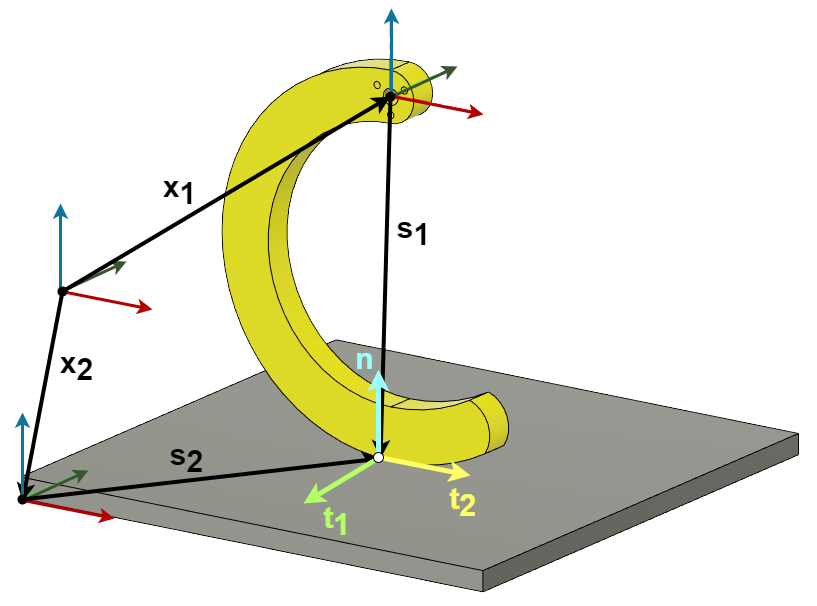
\includegraphics[height=6cm,width=1\textwidth,keepaspectratio]{contact_interaction.png}
                \label{fig:contact_interaction.png}
            \end{figure}
            \vspace{-1cm}
            \begin{align}
                \left\{\begin{matrix*}[l]
                           \mu f_n \geqslant \sqrt{f_1^2 + f_2^2}\\
                           \left\lVert \vec{v_t}\right\rVert (\mu f_n - \sqrt{f_1^2 + f_2^2}) = 0\\
                           \dfrac{\vec{f_t}}{\left\lVert \vec{f_t}\right\rVert } = - \dfrac{\vec{v_t}}{\left\lVert \vec{v_t}\right\rVert }
                       \end{matrix*}\right.
            \end{align}
        \end{column}
    \end{columns}
\end{frame}

\begin{frame}[t]{Закономерность}

    \begin{columns}[T,onlytextwidth]
        \begin{column}{0.49\textwidth}
            Лучшие роботы в экспериментах начинались с 8 до 14 ног для различных значений $\omega$.

            Это объясняется критерием статического равновесия. В таком случае минимум 4 ноги всегда касаются поверхности.
        \end{column}
        \begin{column}{0.49\textwidth}
            \begin{figure}[H]
                \centering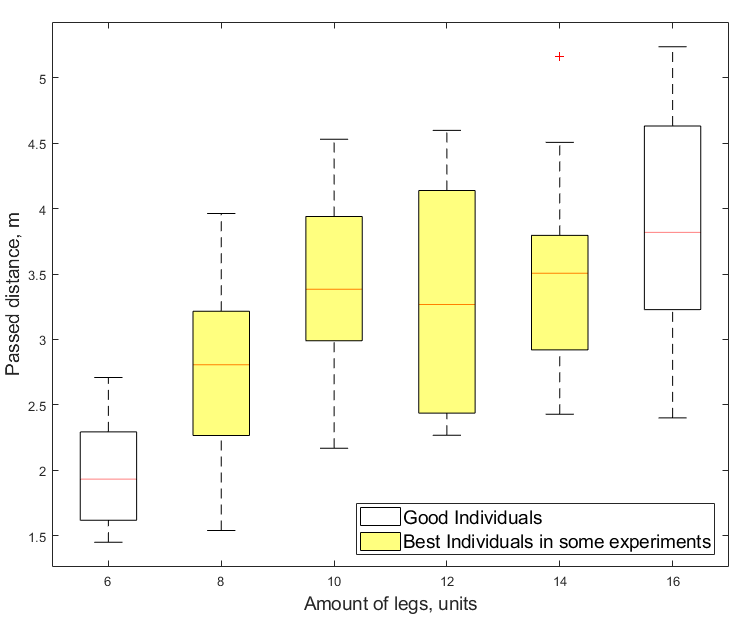
\includegraphics[height=5cm,width=1\textwidth,keepaspectratio]{box_plot_structural_synthesis.png}
                \caption*{Зависимость между кол-вом ног и пройденной дистанцией}
            \end{figure}
        \end{column}
    \end{columns}
\end{frame}

\begin{frame}[c]{Прототипы робота}
    \begin{figure}[H]
        \begin{subfigure}{0.32\textwidth}
            \centering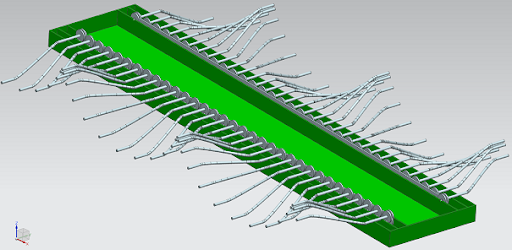
\includegraphics[height=3cm,width=1\textwidth,keepaspectratio]{strirus_0.png}
        \end{subfigure}
        \begin{subfigure}{0.32\textwidth}
            \centering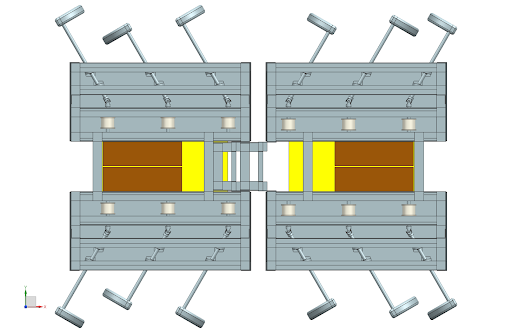
\includegraphics[height=3cm,width=1\textwidth,keepaspectratio]{strirus_1.png}
        \end{subfigure}
        \begin{subfigure}{0.32\textwidth}
            \centering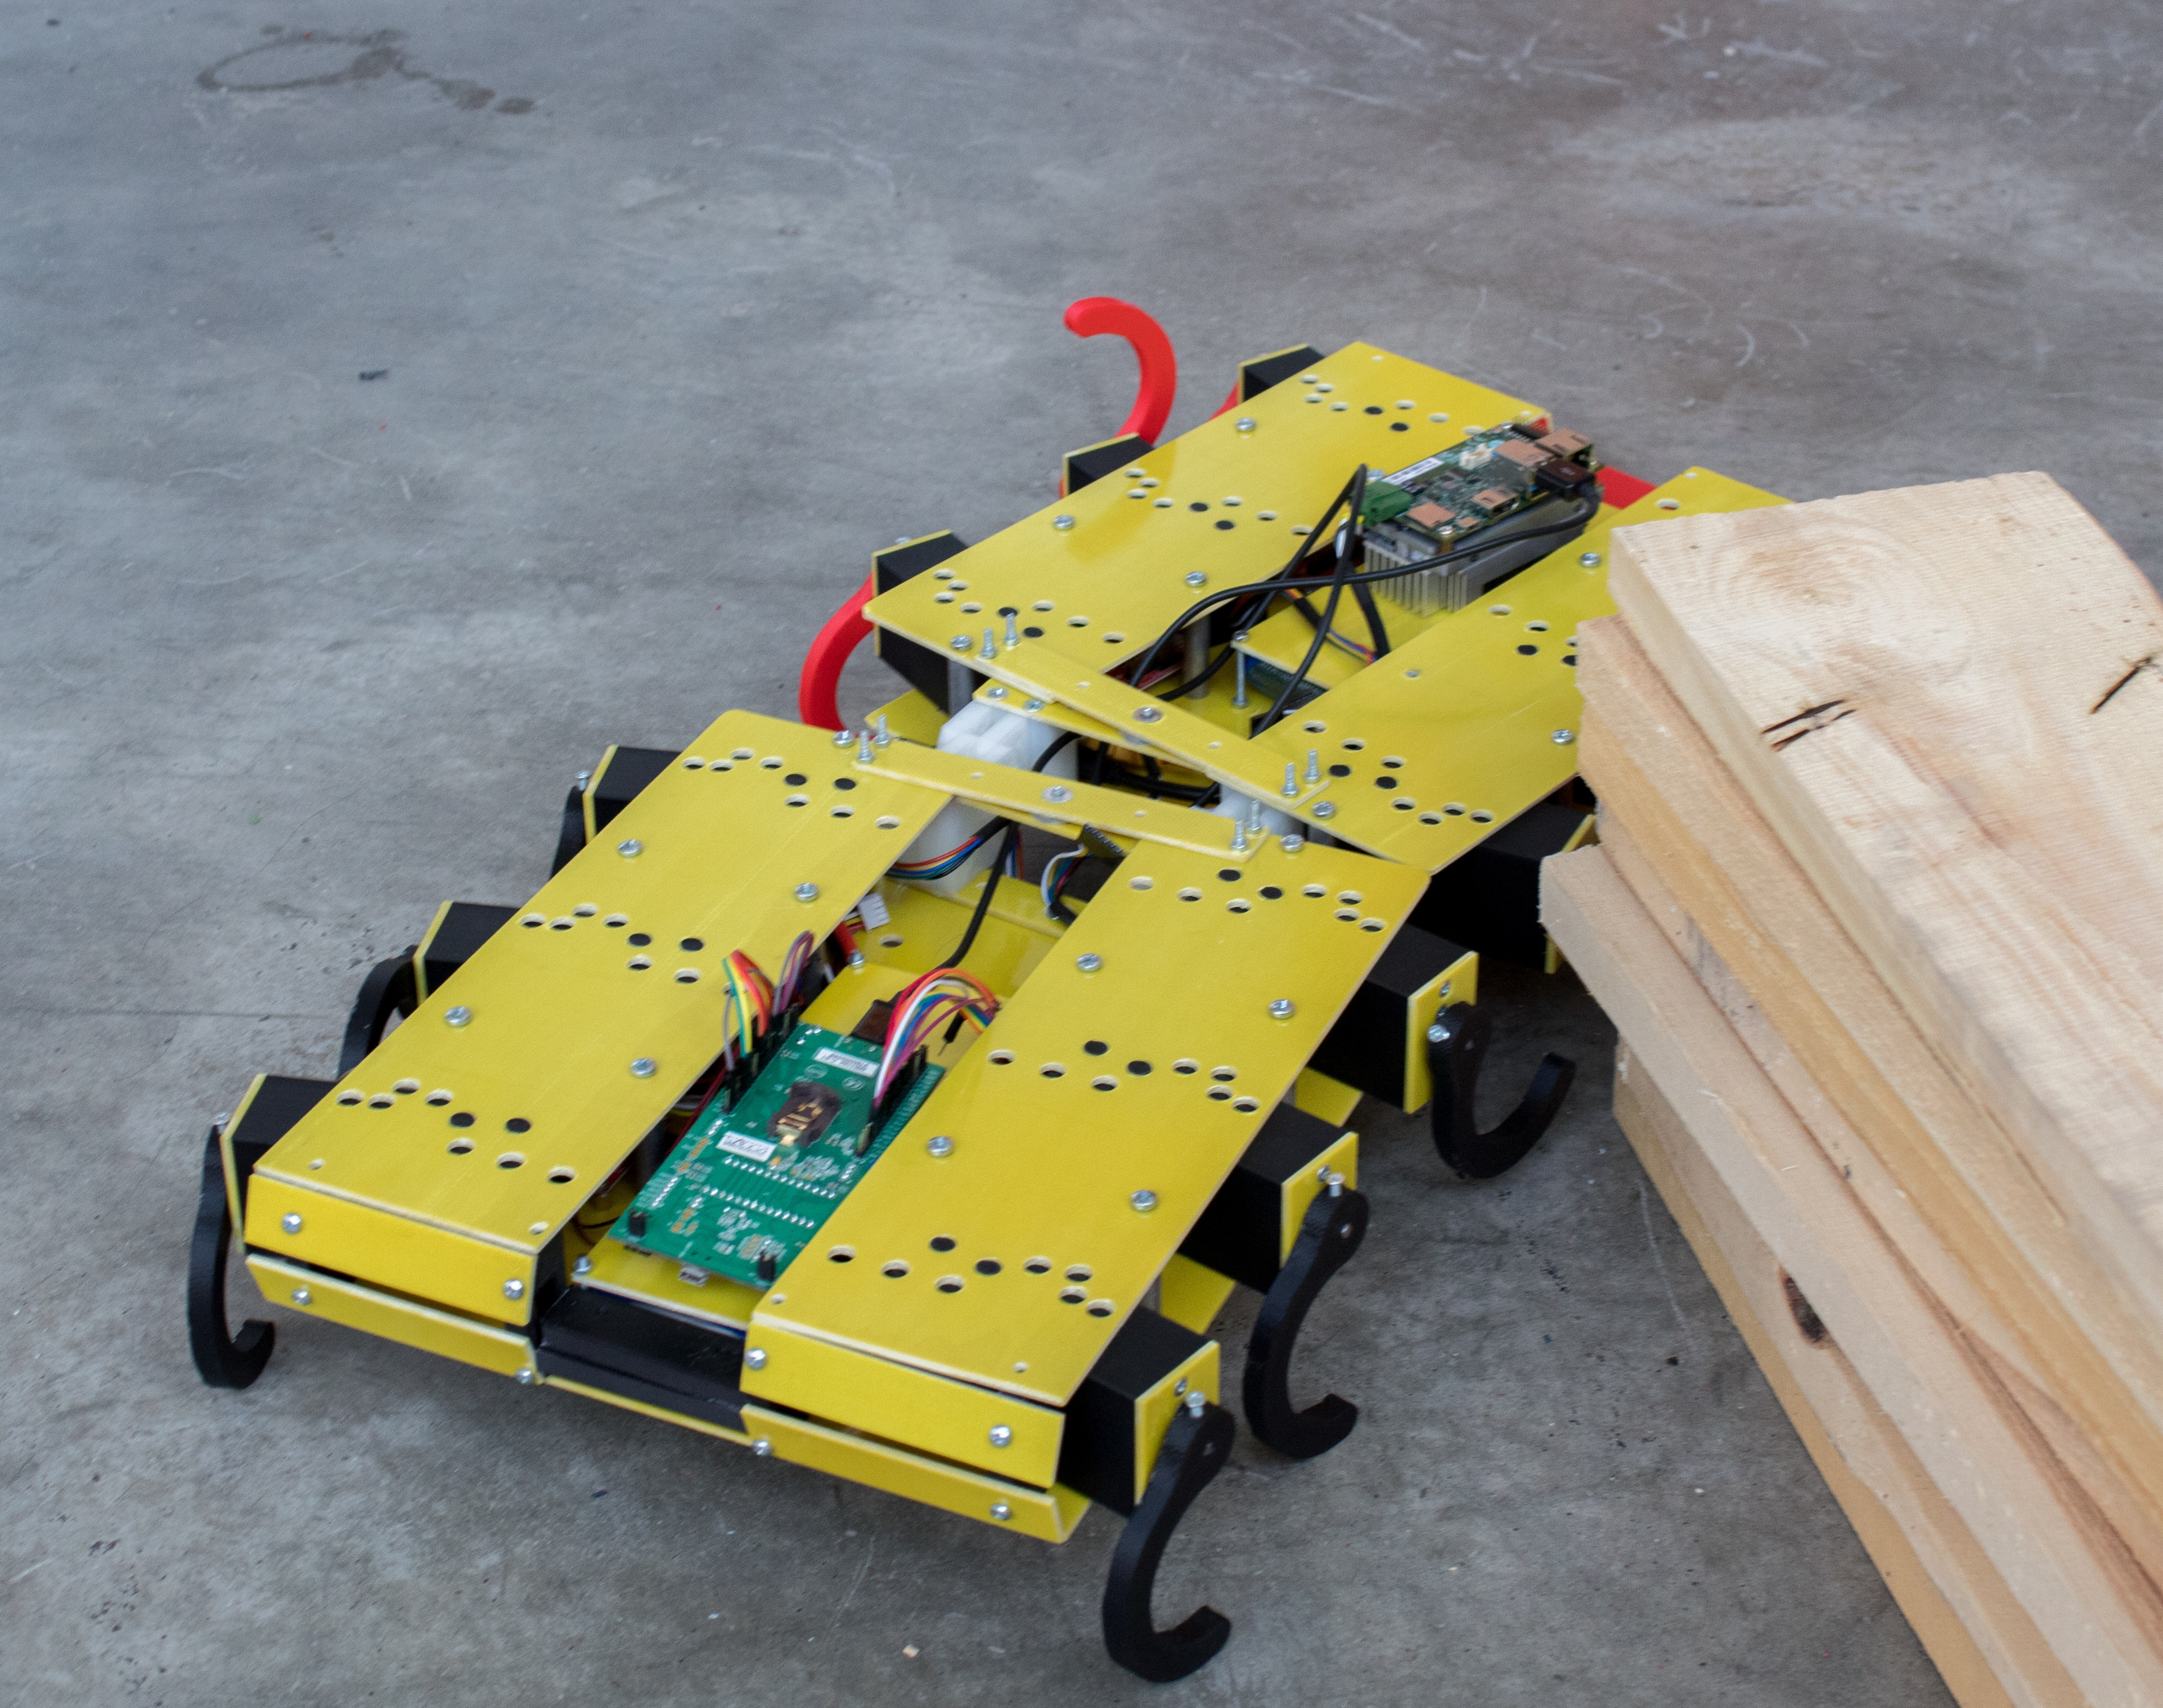
\includegraphics[height=3cm,width=1\textwidth,keepaspectratio]{strirus_2.jpg}
        \end{subfigure}

        \begin{subfigure}{0.32\textwidth}
            \centering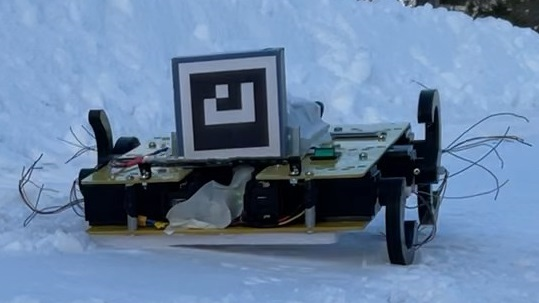
\includegraphics[height=3cm,width=1\textwidth,keepaspectratio]{strirus_3_snow.jpg}
        \end{subfigure}
        \begin{subfigure}{0.32\textwidth}
            \centering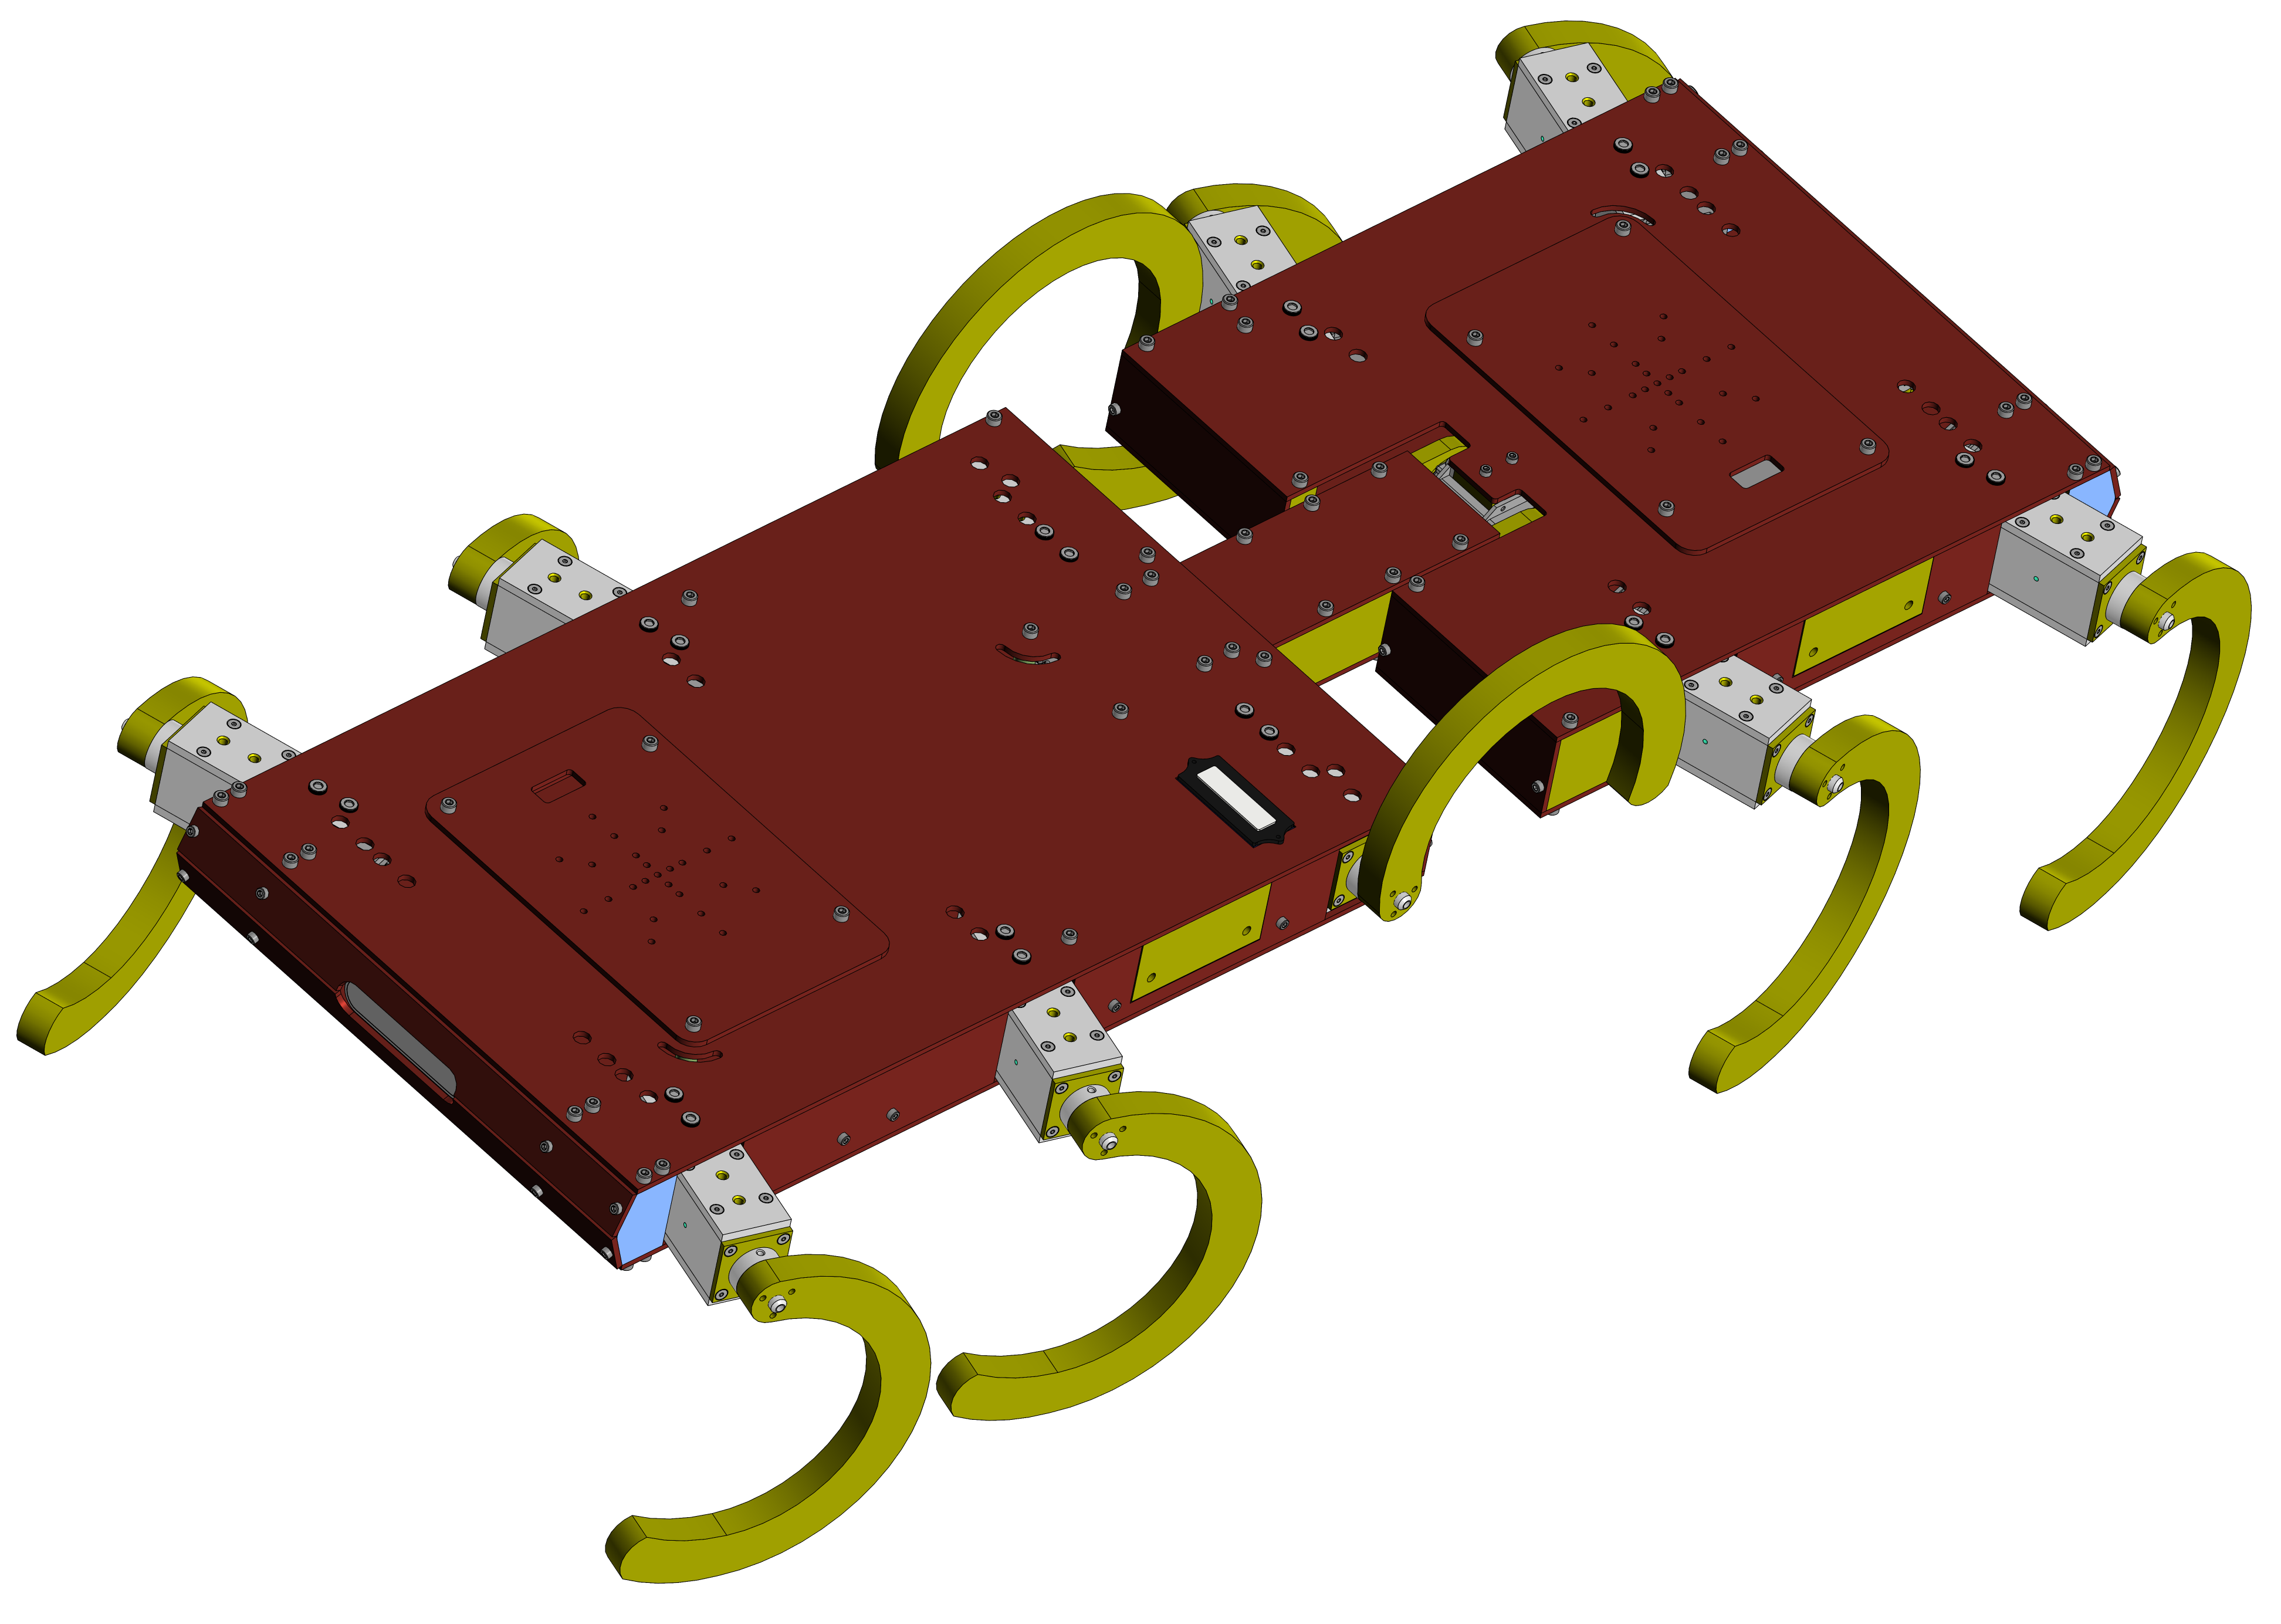
\includegraphics[height=3cm,width=1\textwidth,keepaspectratio]{strirus_4.png}
        \end{subfigure}
    \end{figure}
\end{frame}

\begin{frame}[c]{Особенности конструкции}
    \framesubtitle{}
    \begin{figure}[H]
        \begin{subfigure}{0.39\textwidth}
            \centering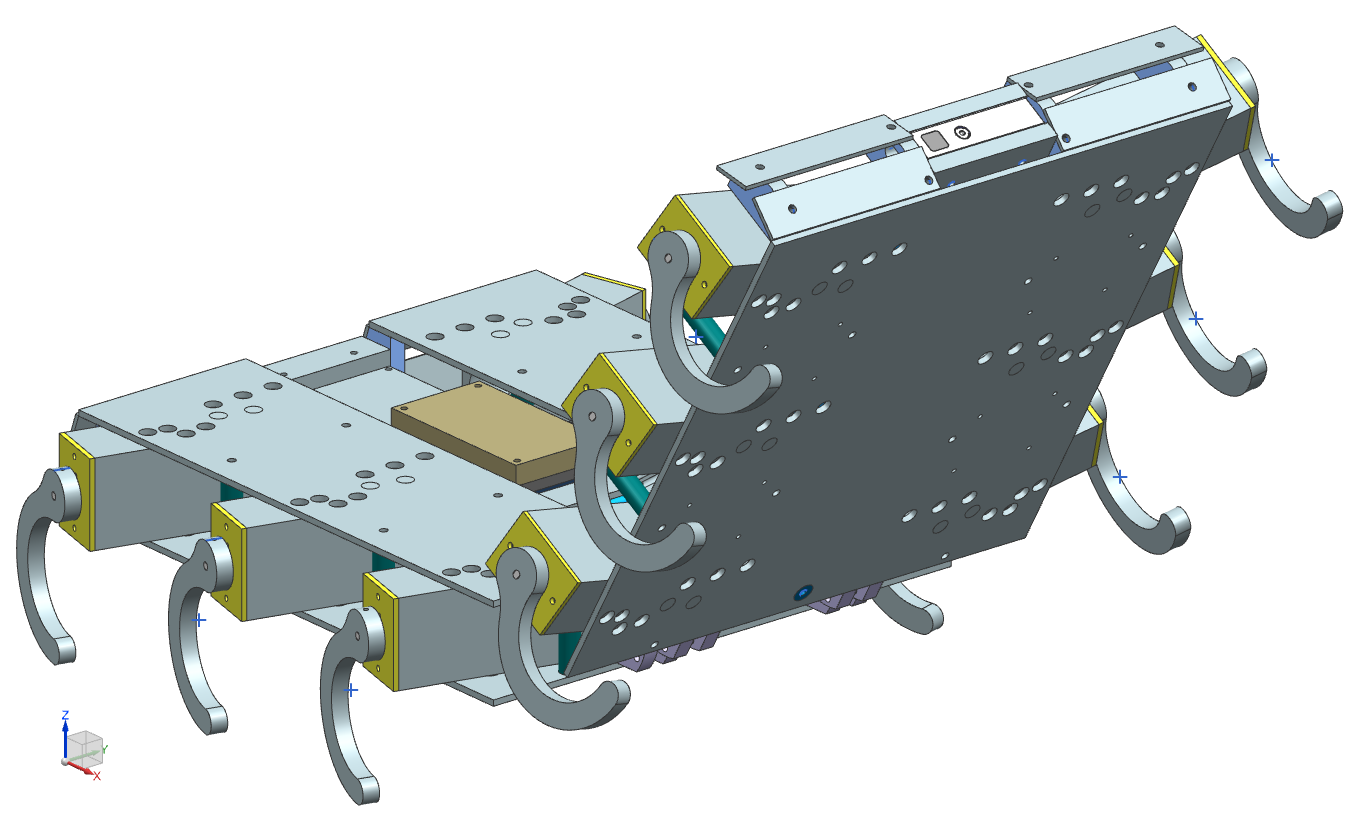
\includegraphics[height=6cm,width=1\textwidth,keepaspectratio]{17.png}
            \caption{Одностепенной активный сегмент, соединяющий 2 части робота}
        \end{subfigure}
        \begin{subfigure}{0.59\textwidth}
            \centering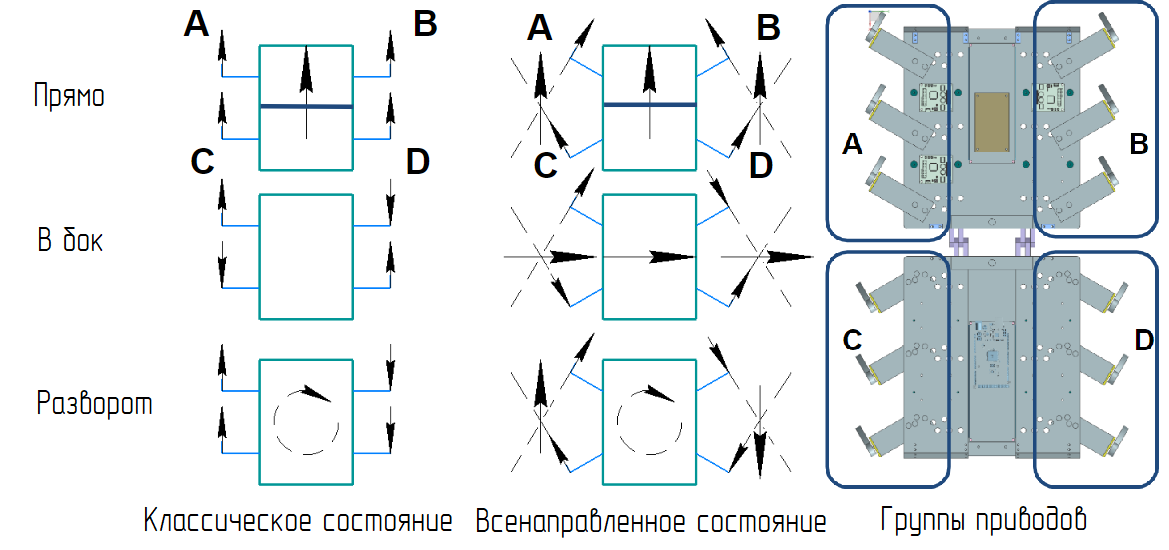
\includegraphics[height=6cm,width=1\textwidth,keepaspectratio]{vector_representation_rus}
            \caption{Векторное представление сил в обычном и всенаправленном состояниях}
        \end{subfigure}
    \end{figure}
\end{frame}

\begin{frame}[t]{Четвертая итерация робота}
    \framesubtitle{}
    \begin{figure}[H]
        \centering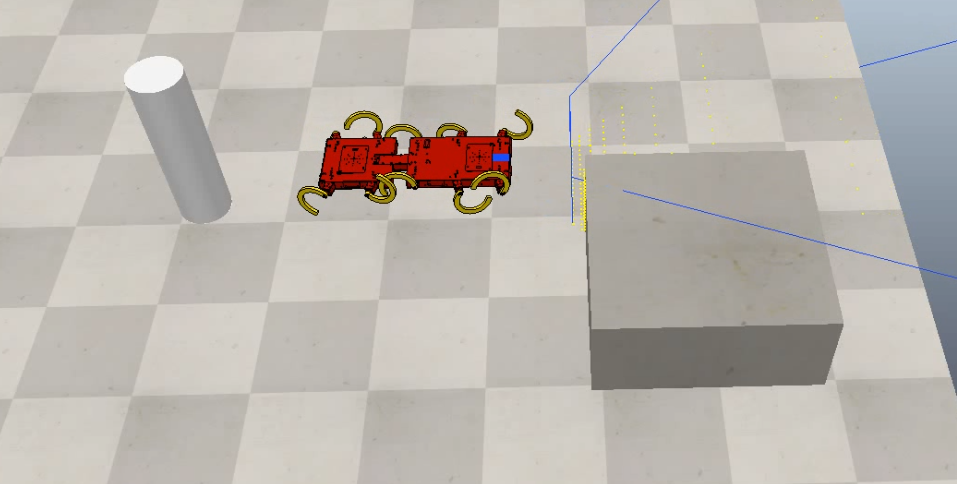
\includegraphics[height=6cm,width=1\textwidth,keepaspectratio]{sidestep_segment_video_preview.png}
    \end{figure}
\end{frame}

\section{"4" Верификация преобразователя силы}

\begin{frame}[t]{Верификация преобразователя силы}
\framesubtitle{}
\begin{columns}[T,onlytextwidth]
\begin{column}{0.69\textwidth}
    \small
    Охарактеризовать материал для случаев, когда площадь приложения силы меньше, чем площадь активной части сенсора.

    \textbf{Идея решения}: Разработка двух экспериментов: 
    
    1. Статический --- прикладывается статический груз с размером в сенсор для \underline{калибровки}.\\
    2. Динамический --- чувствительная область представляется в виде сетки $4\times4$. Происходит касание каждой области с одинаковым давлением, но разной площадью контакта.

    \textbf{Входные данные}: показания разработанного датчика и значение реально приложенной нагрузки.

    \textbf{Выходные данные}: разница между нормализованным значением с датчика и реальной нагрузкой.

    \textbf{Допустимая ошибка}: 10\%

    \textbf{Предположения}: 1) материал обладает вязко-эластичными свойствами, поэтому надо учитывать гистерезис.
\end{column}
\begin{column}{0.29\textwidth}
\begin{figure}[H]
\begin{subfigure}{0.99\textwidth}
    \centering
    \begin{tikzpicture}
        % Include the image in a node
        \node [above right, inner sep=0] (image) at (0,0)
        {\centering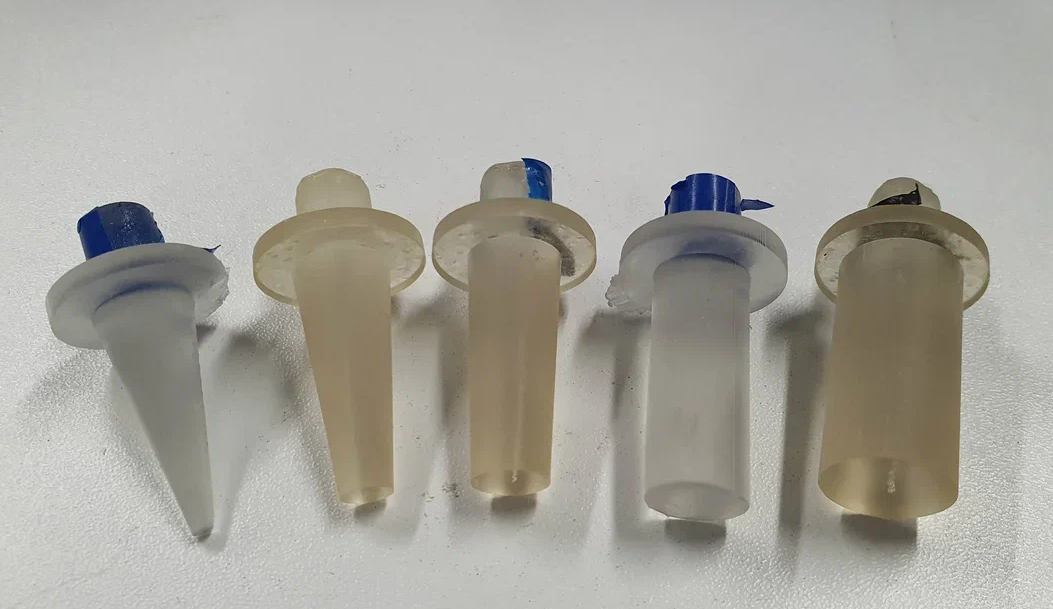
\includegraphics[height=3cm,width=1\textwidth,keepaspectratio]{all_end_effectors.png}};
        % Create scope with normalized axes
        \begin{scope}[
                x={($ 0.1*(image.south east)$)},
                y={($ 0.1*(image.north west)$)}]
            % Labels
            \node[rounded corners=3pt,black,fill=white] at (1.1,7.4){\tiny 2 мм };
            \node[rounded corners=3pt,black,fill=white] at (3.1,7.9){\tiny 6 мм };
            \node[rounded corners=3pt,black,fill=white] at (4.9,8.1){\tiny 8 мм };
            \node[rounded corners=3pt,black,fill=white] at (6.7,7.9){\tiny 12 мм };
            \node[rounded corners=3pt,black,fill=white] at (8.6,7.9){\tiny 15 мм };
        \end{scope}
    \end{tikzpicture}
    \caption{Все насадки}
\end{subfigure}

\begin{subfigure}{0.99\textwidth}
    \centering
    \begin{tikzpicture}
        % Include the image in a node
        \node [
            above right,
            inner sep=0] (image) at (0,0) {\centering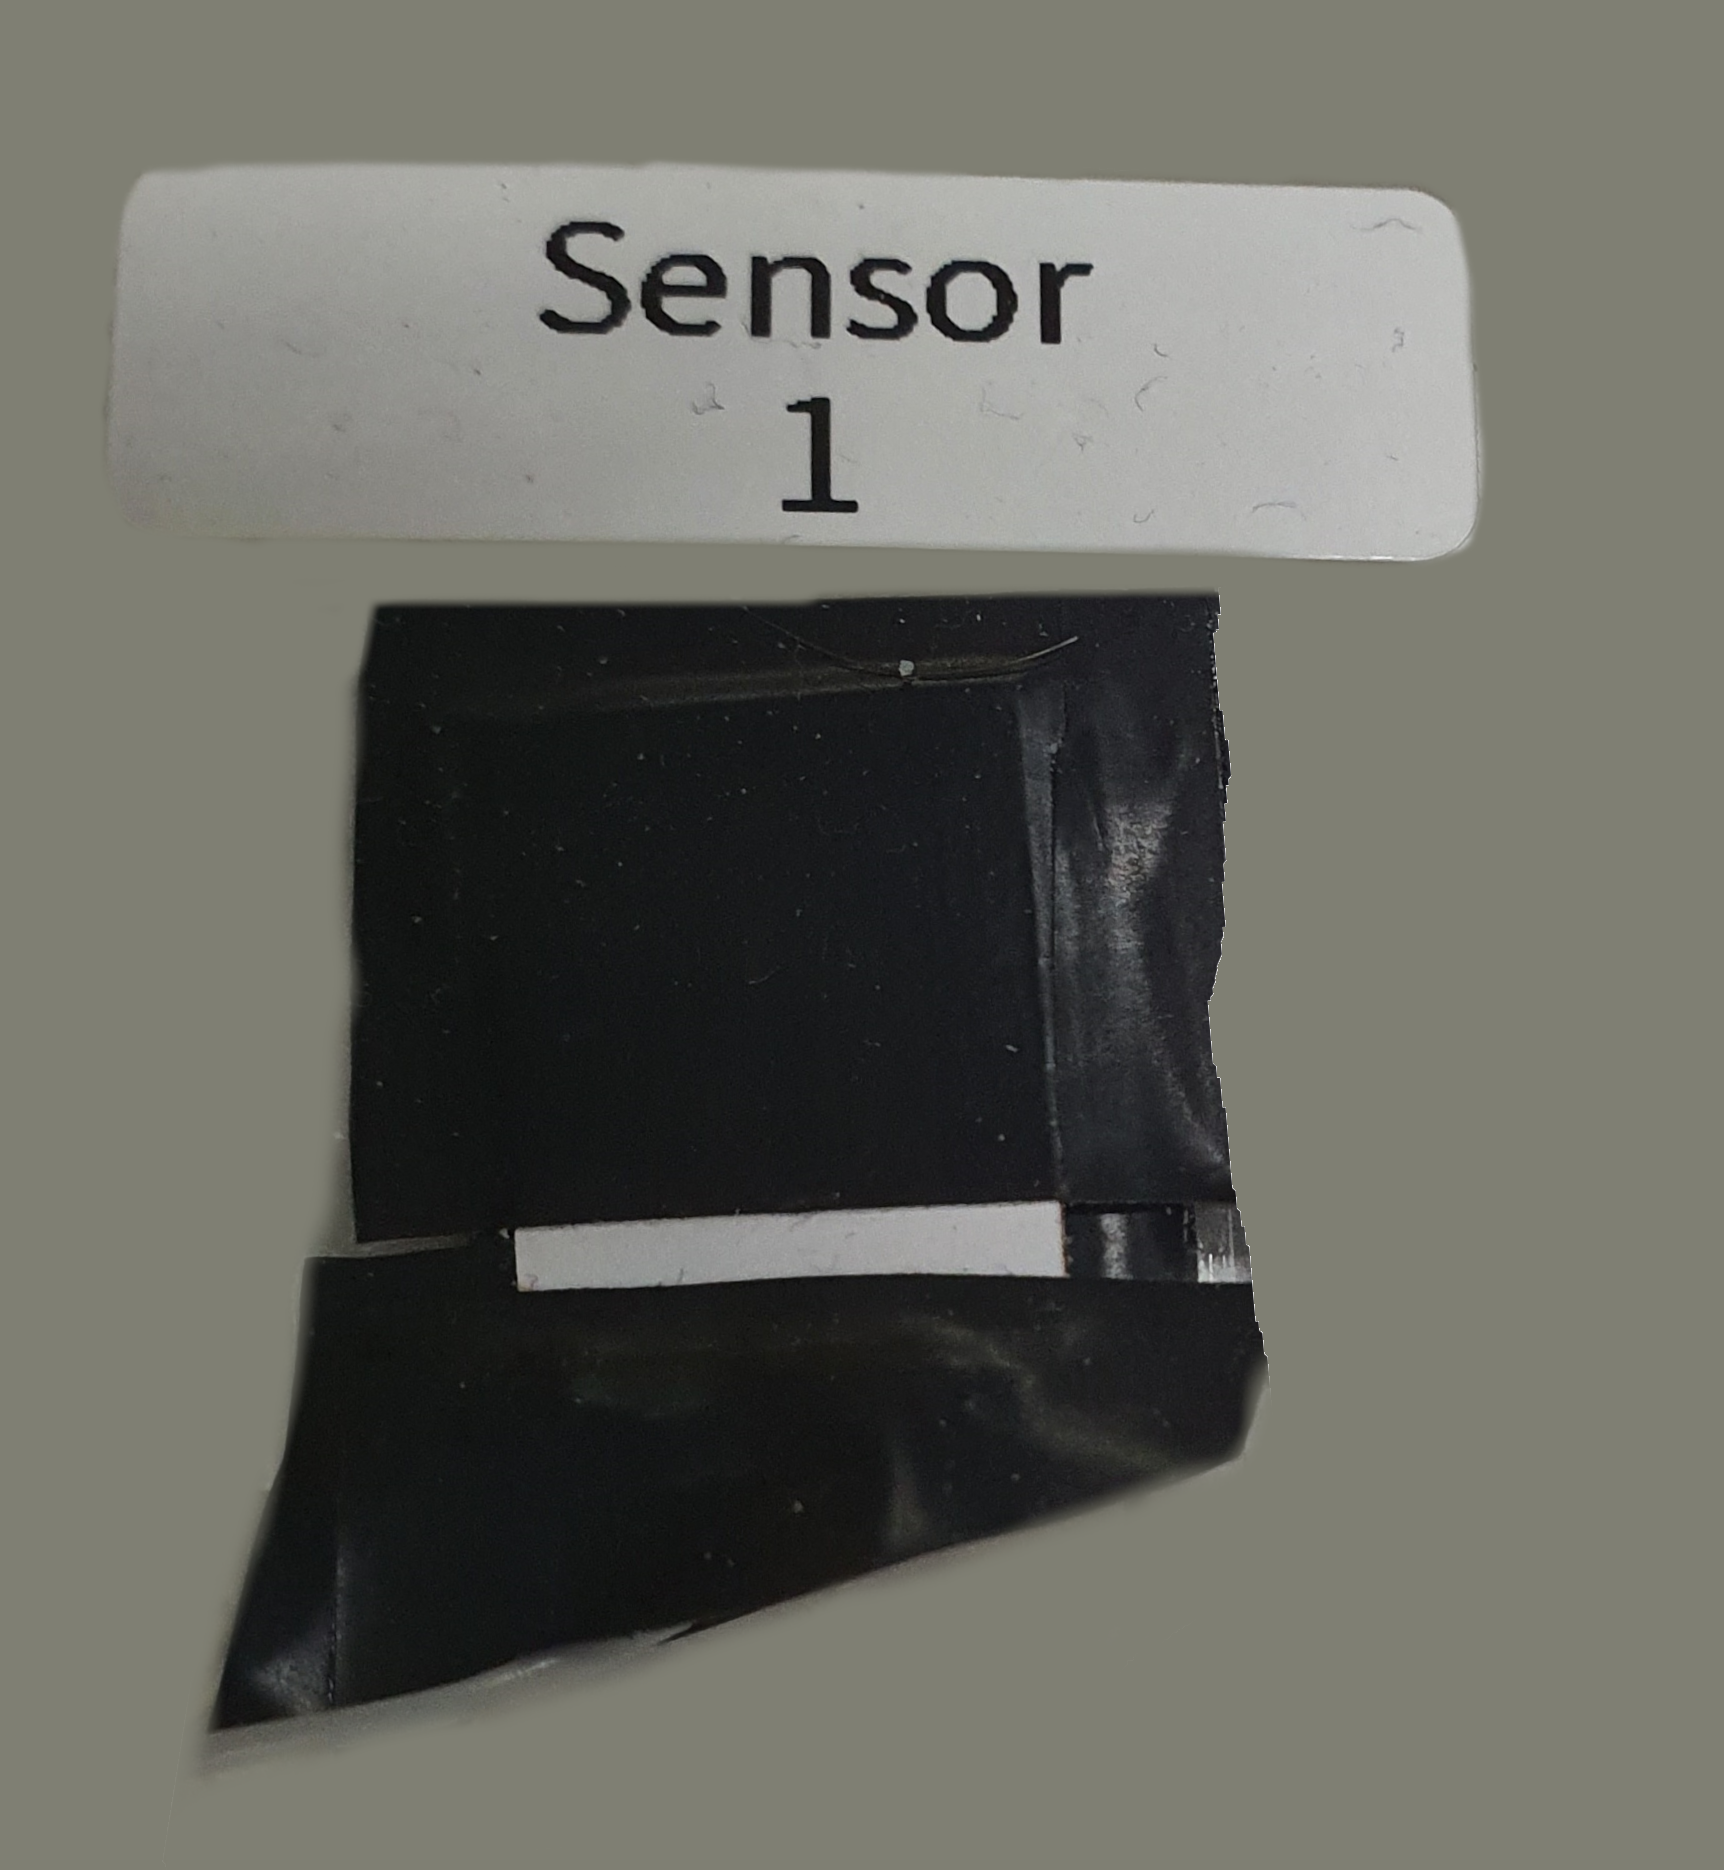
\includegraphics[height=3cm,width=1\textwidth,keepaspectratio]{sensors_grid.png}};

        % Create scope with normalized axes
        \begin{scope}[
                x={($0.1*(image.south east)$)},
                y={($0.1*(image.north west)$)}]
            % Labels
            % Simple brace
            \draw [green, very thick,
                decorate,
                decoration = {brace,
                        raise=5pt,
                        amplitude=5pt,
                        aspect=0.5}] (6,3.7) --  (3,3.7)
            node[pos=0.5,below=10pt,green]{$15\ \text{мм}$};

            \draw [green, very thick,
                decorate,
                decoration = {brace, mirror,
                        raise=5pt,
                        amplitude=5pt,
                        aspect=0.5}] (6,3.6) --  (6,6.4)
            node[pos=0.5,right=10pt,green]{$15\ \text{мм}$};

            \draw[green,step=1,xshift=34, yshift=43]  (0.5,0.5) grid +(3,3);

            \node[circle,fill=green,scale=0.4] at (3.3,6.27){\small 1};
            \node[circle,fill=green,scale=0.4] at (5.92,3.7){\small 16};
        \end{scope}
    \end{tikzpicture}
    \caption{Поверхность \\ как $4\times4$ сетка}
    \end{subfigure}
\end{figure}
\end{column}
\end{columns}
\end{frame}


\begin{frame}[t]{Статический эксперимент}
    \begin{columns}[T,onlytextwidth]
        \begin{column}{0.52\textwidth}
            \begin{eqnarray*}
                V_{out} = V_0 + p[k_p + k_e(1-e^\frac{-(t-t_0)}{\tau_{res}})](1-e^{-\frac{A}{p}}) \\
                k_p = A_1e^{-A_2p}; \tau_{res} = B_0 + B_1e^{-\frac{p}{B_2}}
            \end{eqnarray*}
            Где $V_0$ -- начальное напряжение, \\ $p$ -- приложенное давление, \\ $A_i,\ B_i,\ \tau_{res},\ k_i$ искомые параметры, \\  $t$ -- текущее время, $t_0$ -- время начала нажатия.
            \\ \alert{Апробированна модель для калибровки датчика}
        \end{column}
        \begin{column}{0.45\textwidth}
            \vspace{-15pt}
            \begin{figure}[H]
                \begin{subfigure}{0.99\textwidth}
                    \centering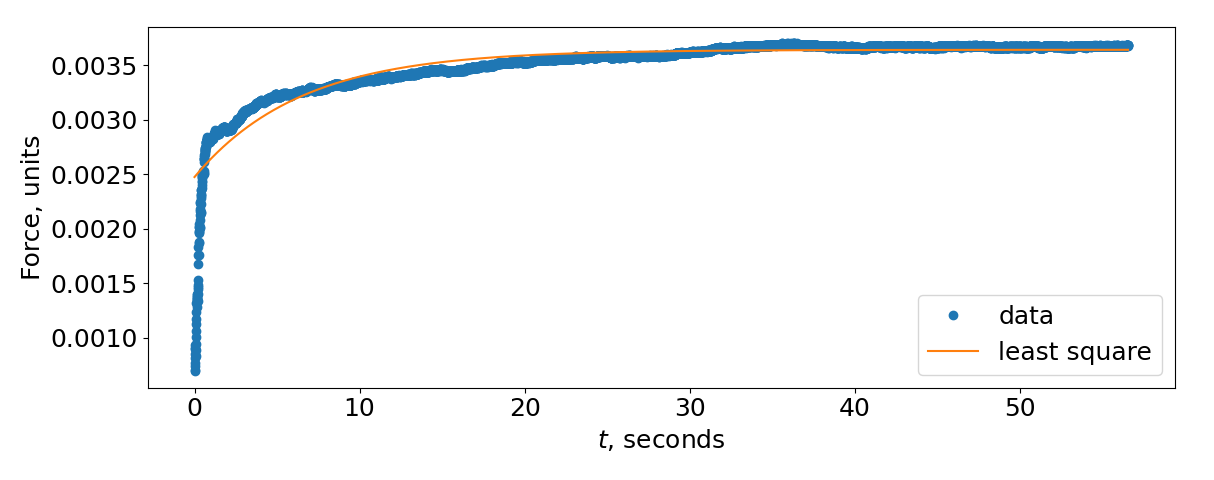
\includegraphics[height=2.8cm,width=1\textwidth,keepaspectratio]{least_square_model.png}
                    \label{fig:least_square_model.png}
                \end{subfigure}
                \vspace{-1cm}

                \begin{subfigure}{0.99\textwidth}
                    \centering
                    \begin{tikzpicture}
                        % Include the image in a node
                        \node [above right, inner sep=0] (image) at (0,0)
                        {\centering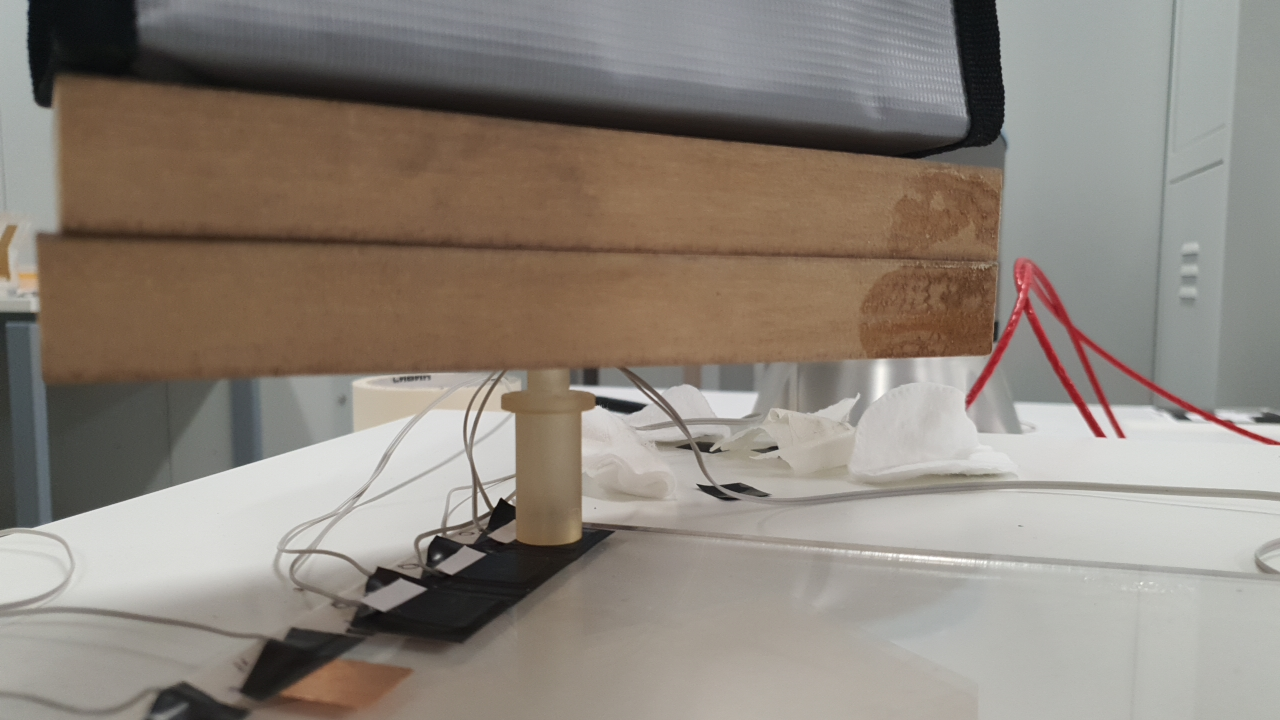
\includegraphics[height=3.4cm,width=1\textwidth,keepaspectratio]{static_load_meh.JPG}};
                        % Create scope with normalized axes
                        \begin{scope}[
                                x={($ 0.1*(image.south east)$)},
                                y={($ 0.1*(image.north west)$)}]
                            \draw[latex-, very thick,green] (4.3,2.3) -- (5,1.6)
                            node[rounded corners=3pt,below right,black,fill=white]{\tiny Исследуемый датчик};

                            \draw[latex-, very thick,green] (4.3,3.5) -- (5.5,2.45)
                            node[rounded corners=3pt,right,black,fill=white]{\tiny \O \ 15 мм насадка};

                            \draw[latex-, very thick,green] (6,6) -- (6.4,4.9)
                            node[rounded corners=3pt,below right,black,fill=white]{\tiny Известная нагрузка};
                        \end{scope}
                    \end{tikzpicture}
                    % \caption*{}
                \end{subfigure}
            \end{figure}
        \end{column}
    \end{columns}
\end{frame}

\begin{frame}[t]{Динамический эксперимент: установка}
    \begin{columns}[T,onlytextwidth]
        \begin{column}{0.39\textwidth}
            \begin{itemize}
                \item Управление силой нажатия {\\ \alert{Импедансное управления}}
                \item Повторяемость эксперимента по силе и позиции{\\ \alert{Добавив манипулятор и камеру}}
                \item Возможность нажимать только на часть сенсора{\\ \alert{Насадки для манипулятора}}
            \end{itemize}
        \end{column}
        \begin{column}{0.8\textwidth}
            \scalebox{0.81}{
                \begin{tikzpicture}

                    % Include the image in a node
                    \node [
                        above right,
                        inner sep=0] (image) at (0,0) {\centering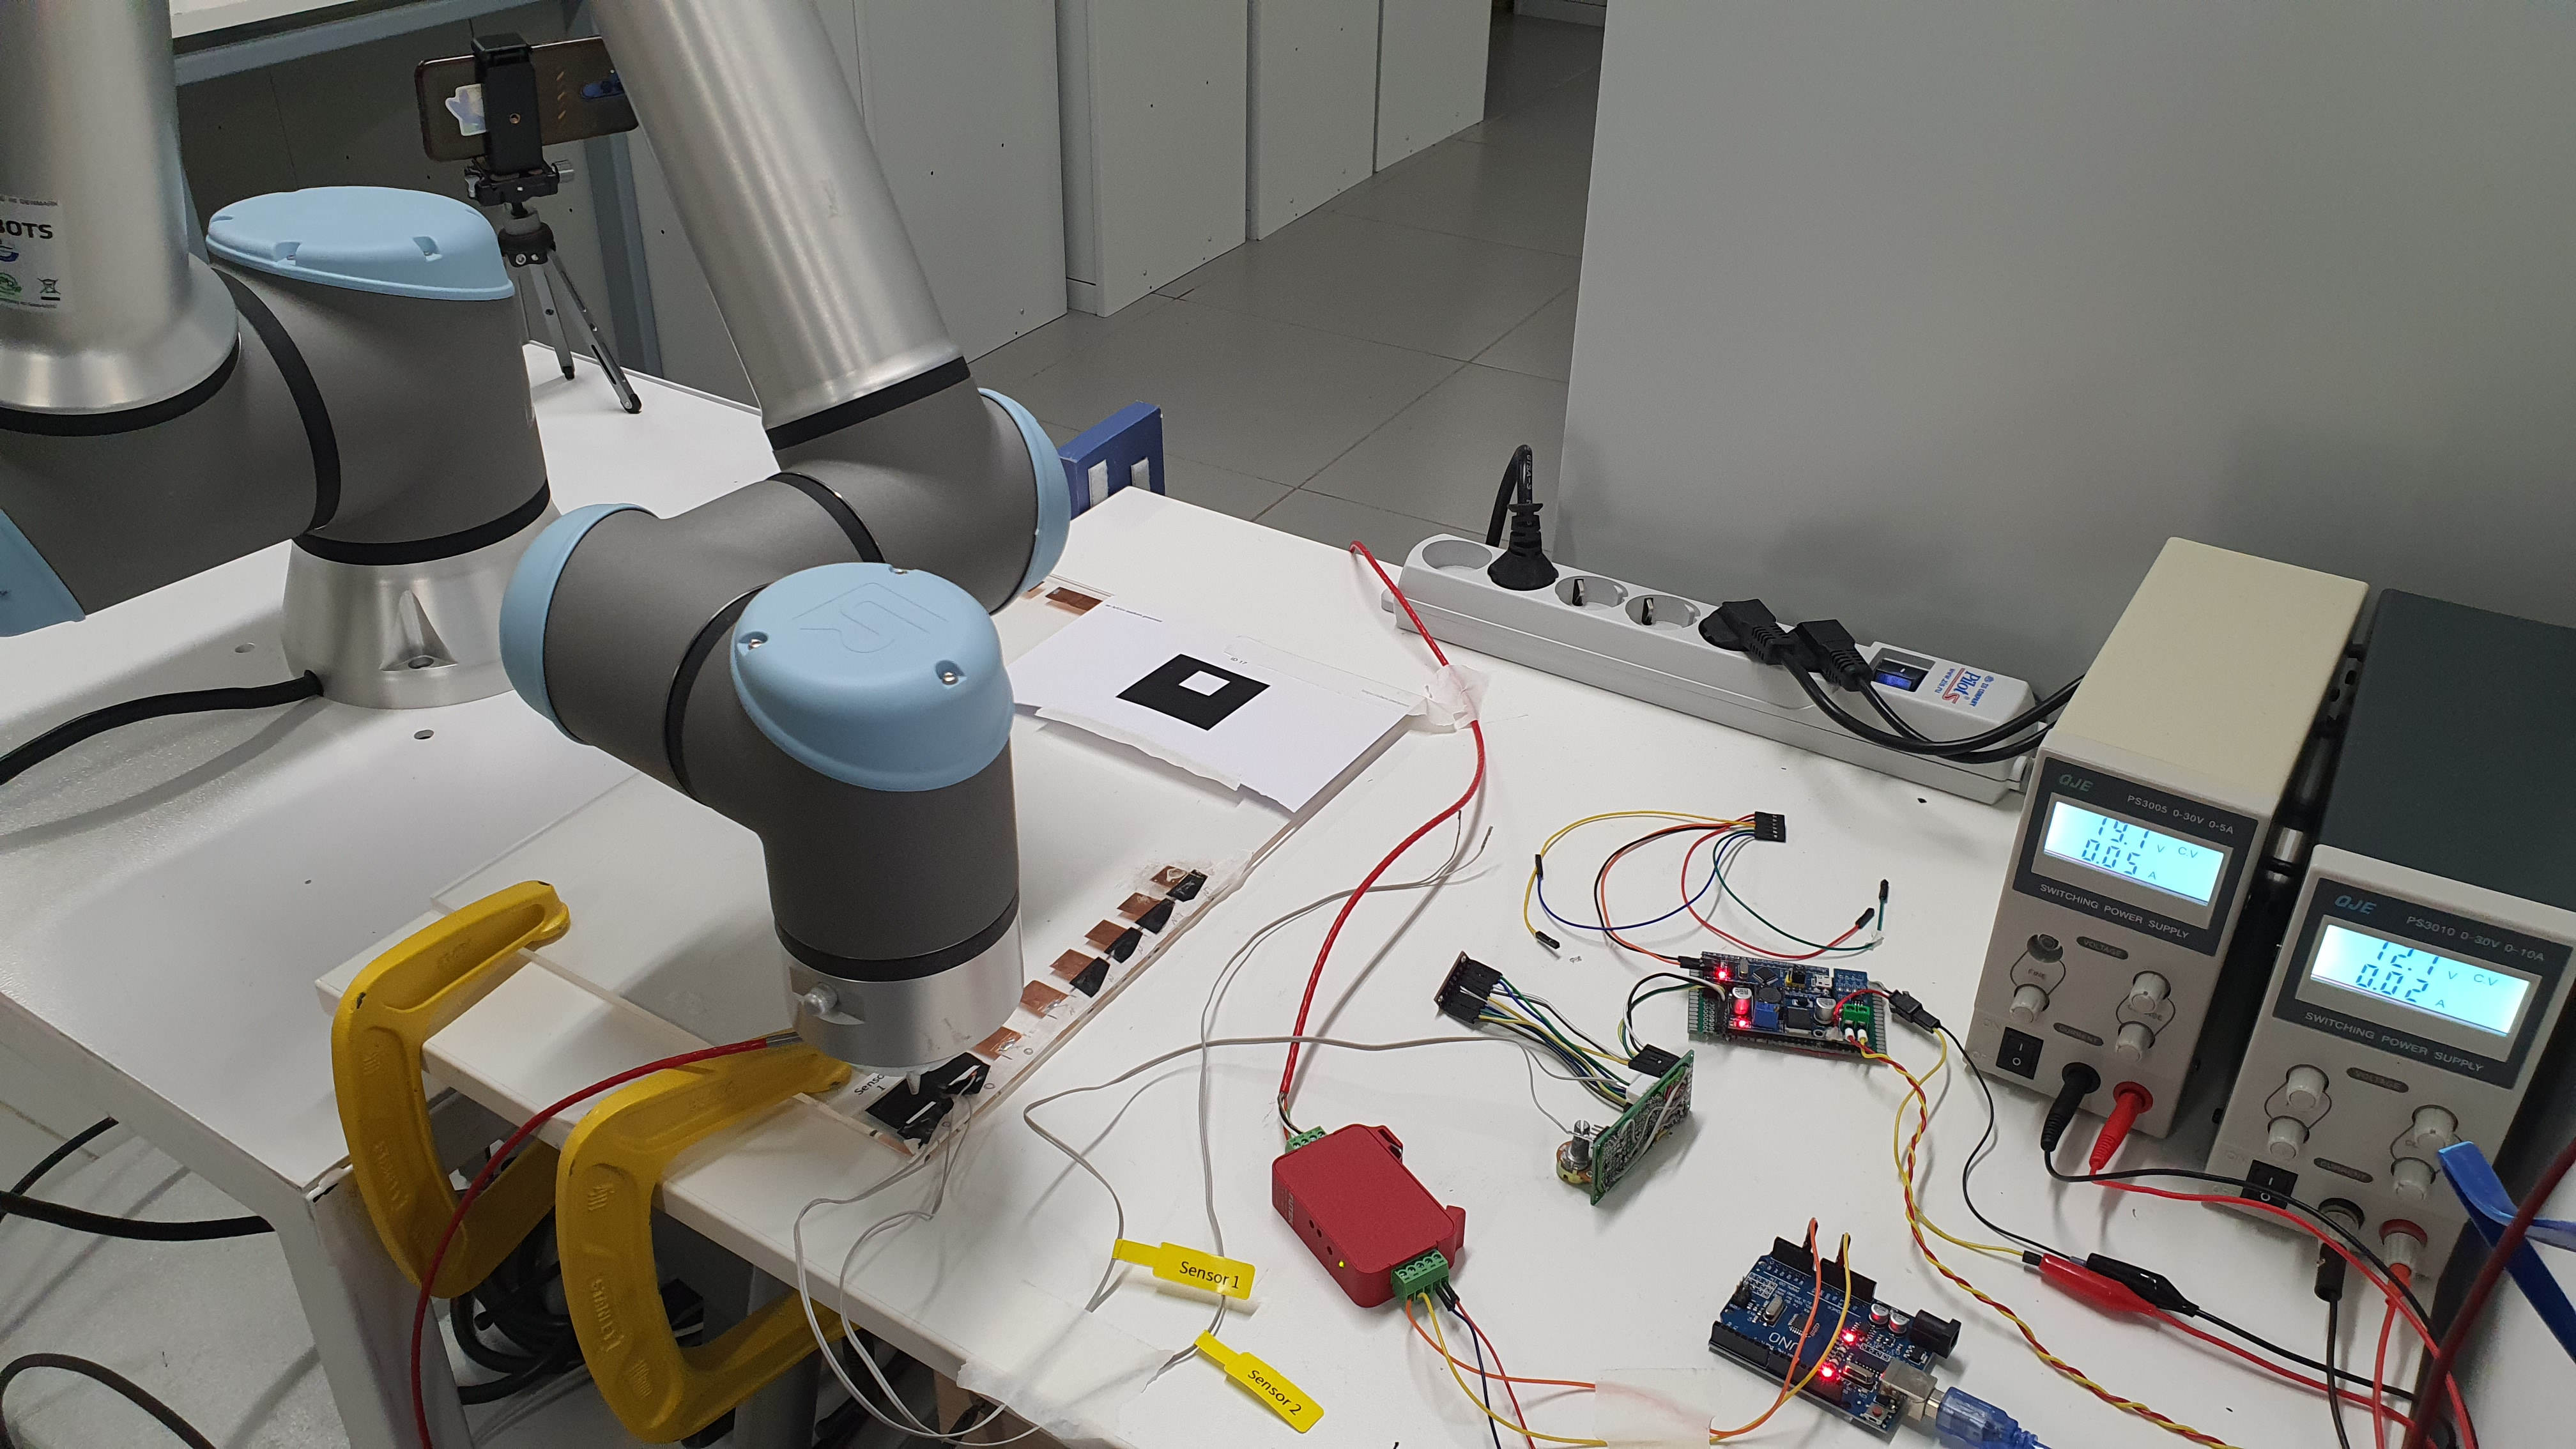
\includegraphics[height=6cm,width=1\textwidth,keepaspectratio]{exp_stand1}};

                    % Create scope with normalized axes
                    \begin{scope}[
                            x={($0.1*(image.south east)$)},
                            y={($0.1*(image.north west)$)}]
                        \draw[latex-, very thick,green] (3.5,2.2) -- (3.5,1)
                        node[rounded corners=3pt,below left,black,fill=white]{\small Исследуемые датчики};

                        \draw[stealth-, very thick,green] (3.5,2.6) -- ++(-0.7,+0.5)
                        node[rounded corners=3pt,left,black,fill=white]{\small Датчик силы};

                        \draw[stealth-, very thick,green] (6.5,3) -- (7,6)
                        node[rounded corners=3pt,above right,black,fill=white]{\small Печатная плата};

                        \draw[stealth-, very thick,green] (7.2,1.5) -- (8,5)
                        node[rounded corners=3pt,above right,black,fill=white]{\small Контроллер};

                        \draw[stealth-, very thick,green] (2.5,9.5) -- (4,9.5)
                        node[rounded corners=3pt,right,black,fill=white]{\small Камера};

                        \draw[very thick,green] (0.5,2.5) rectangle (4.2,9)
                        node[below left,black,fill=green]{\small UR10e};

                        \draw[latex-, very thick,green] (4.5,7.2) edge (5.5,7.5)
                        (4.8,5.3) -- (5.5,7.5)
                        node[rounded corners=3pt,above,black,fill=white]{\small Маркеры Aruco};
                    \end{scope}

                \end{tikzpicture}
            }
        \end{column}
    \end{columns}
\end{frame}

\begin{frame}[t]{Результаты динамического эксперимента}
    \begin{figure}[H]
        \begin{subfigure}{0.49\textwidth}
            \centering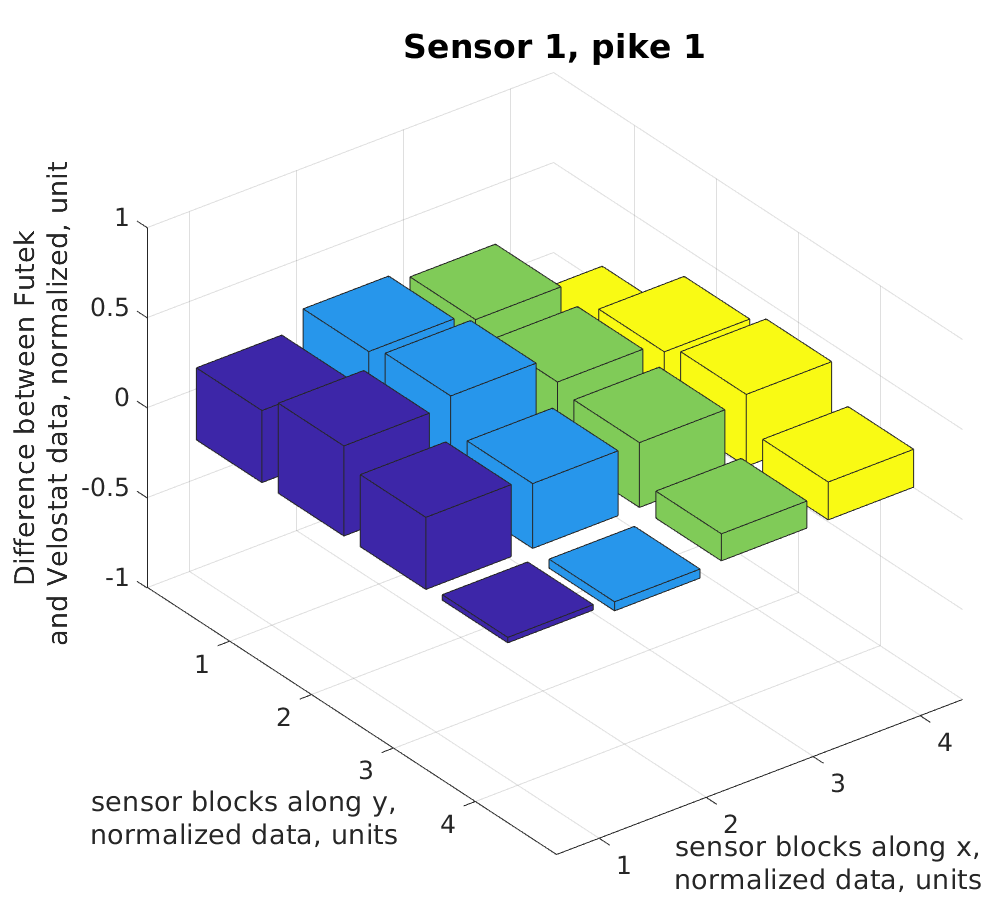
\includegraphics[height=5cm,width=1\textwidth,keepaspectratio]{sens1_pike1.png}
            \caption*{2 мм диаметр насадки}
            \label{fig:sens1_pike1}
        \end{subfigure}
        \begin{subfigure}{0.49\textwidth}
            \centering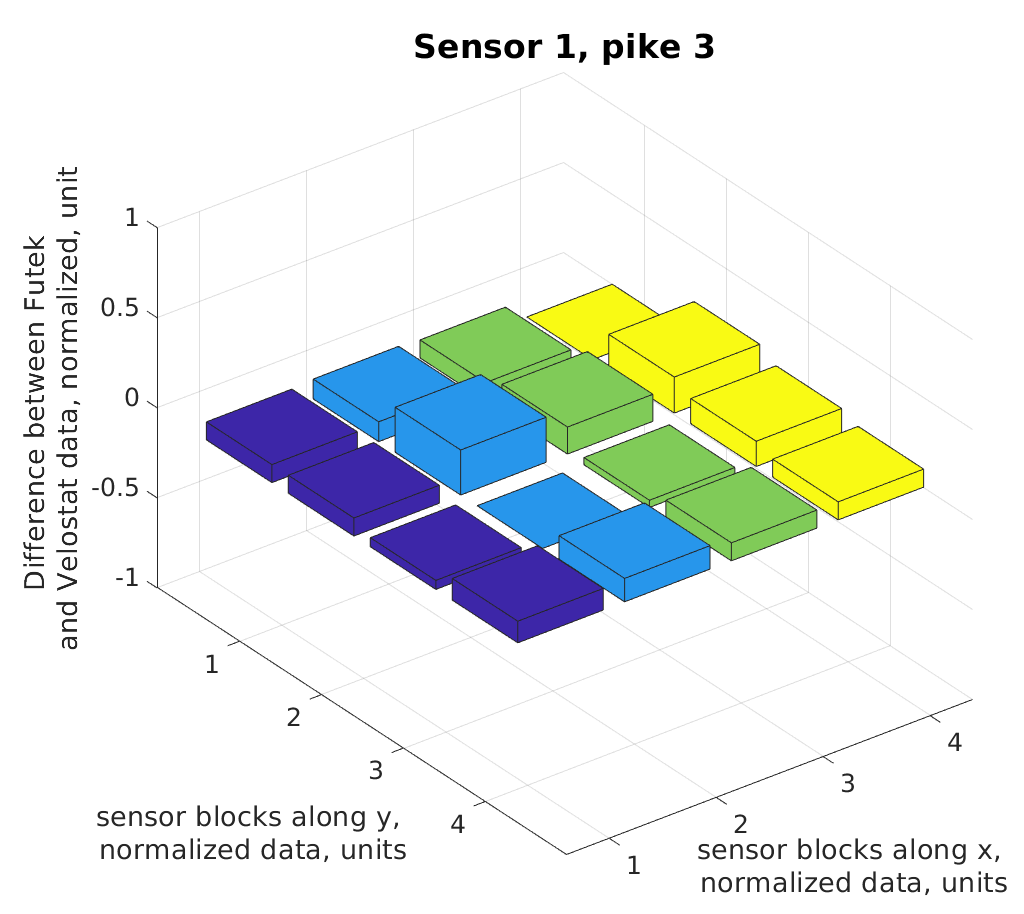
\includegraphics[height=5cm,width=1\textwidth,keepaspectratio]{sens1_pike3.png}
            \caption*{8 мм диаметр насадки}
            \label{fig:sens1_pike3}
        \end{subfigure}
    \end{figure}
    \vspace{-0.8cm}
    \alert{Одинаковые данные, когда площадь нажатия превышает 25\% от площади датчика}
\end{frame}

\section{"2" Определение физико-механических свойств поверхности}

\begin{frame}[t]{Определение физико-механических свойств}
\framesubtitle{}
    \small
    Определить процентное соотношение твердых, упругих и пластичных свойств пройденной поверхности

\textbf{Метод решения}: машинное обучение, Метод Опорных Векторов (SVM) 

\textbf{Идея решения}: Создается установка для обучения. Обучение: робот ходит по различным типам поверхностей фиксированное количество касаний поверхности с постоянной угловой скоростью. Собранные данные разбиваются на 2 части 80\% и 20\%. Модель обучается на 80\% с помощью ядра PUK7. Тестирование: происходит на оставшиеся 20\%.  Используются метрики меткости, точности, полноты и F1-счета.

\begin{columns}[T,onlytextwidth]
    \begin{column}{0.44\textwidth}
        \textbf{Входные данные}: обученный классификатор 
поверхностей, данные с внутренних 
датчиков робота

\textbf{Выходные данные}: процентное 
соотношение упругих, твердых 
и пластичных свойств 
пройденной поверхности

\textbf{Допустимая ошибка}: 20\% - точность

\textbf{Предположения}: 1) На рисунке.

    \end{column}
    \begin{column}{0.54\textwidth}
        \vspace{-0.9cm}
        \begin{figure}[H]
            \begin{subfigure}[b]{0.3\textwidth}
                \centering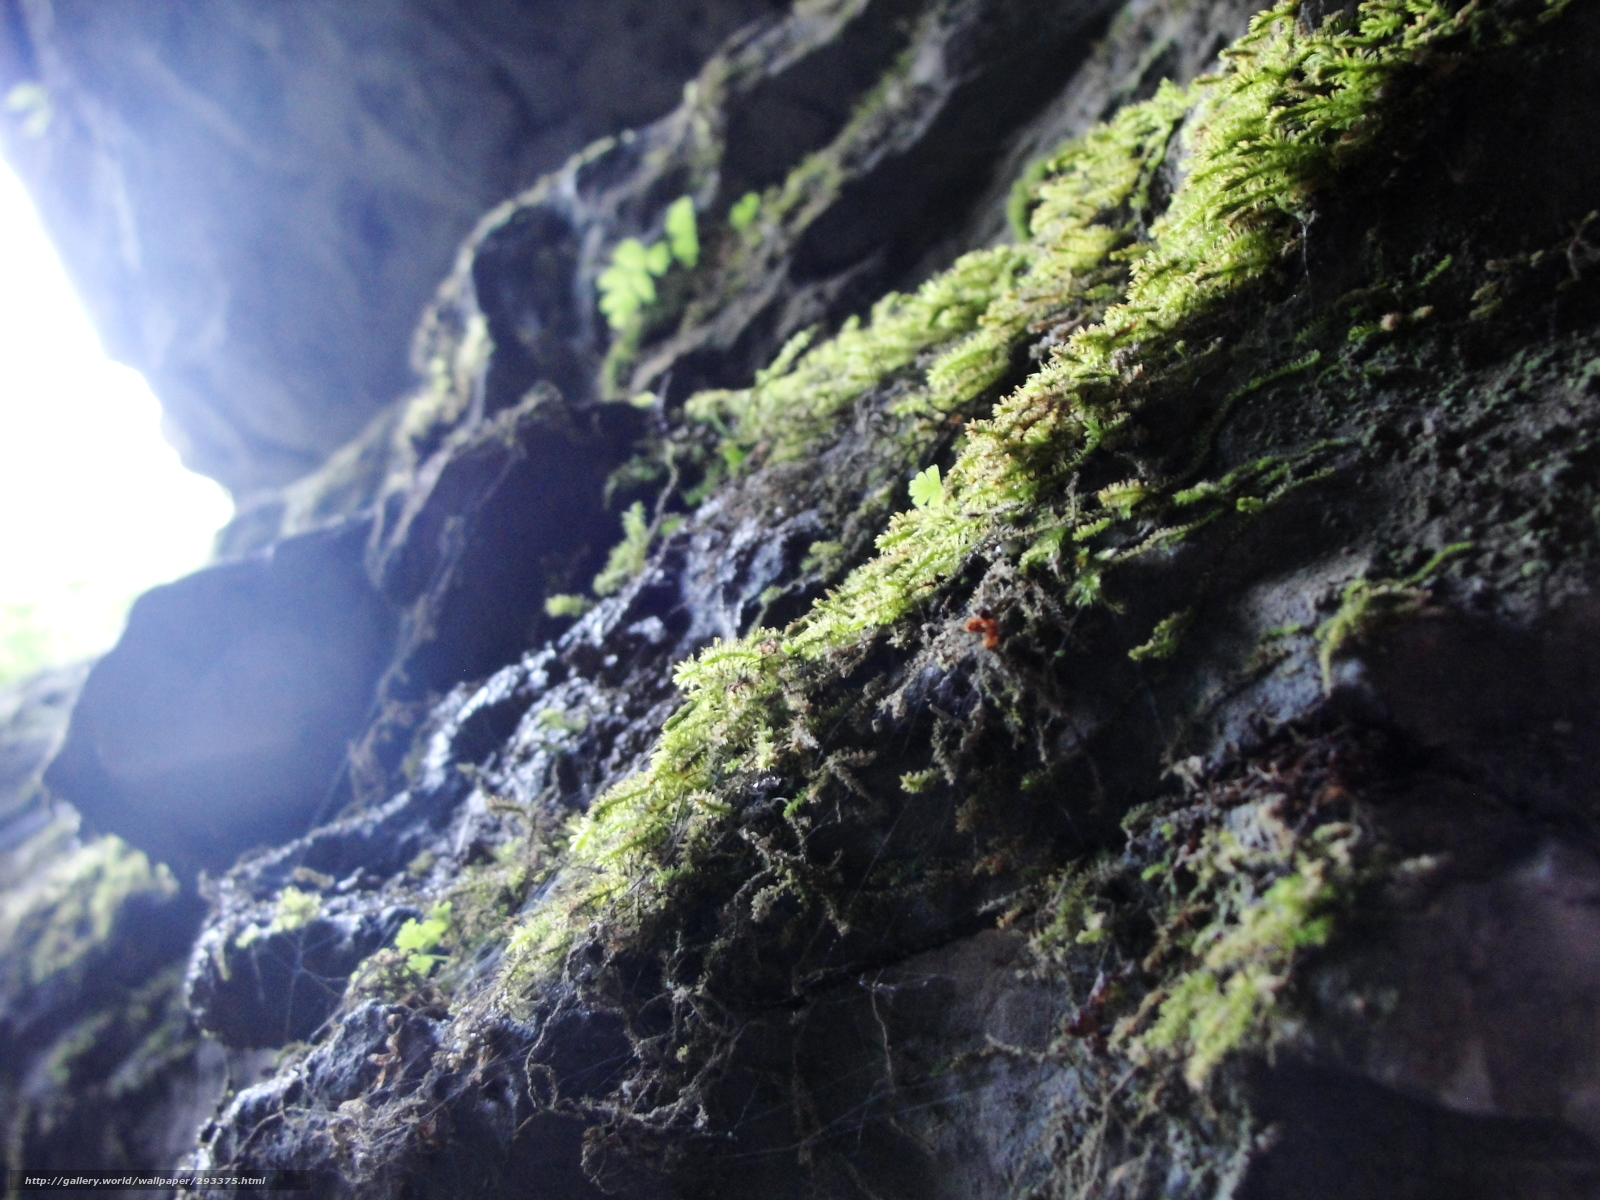
\includegraphics[height=1.5cm,width=1\textwidth,keepaspectratio]{surface_types/moss.jpg}
            \end{subfigure}
            \hfill
            \begin{subfigure}[b]{0.3\textwidth}
                \centering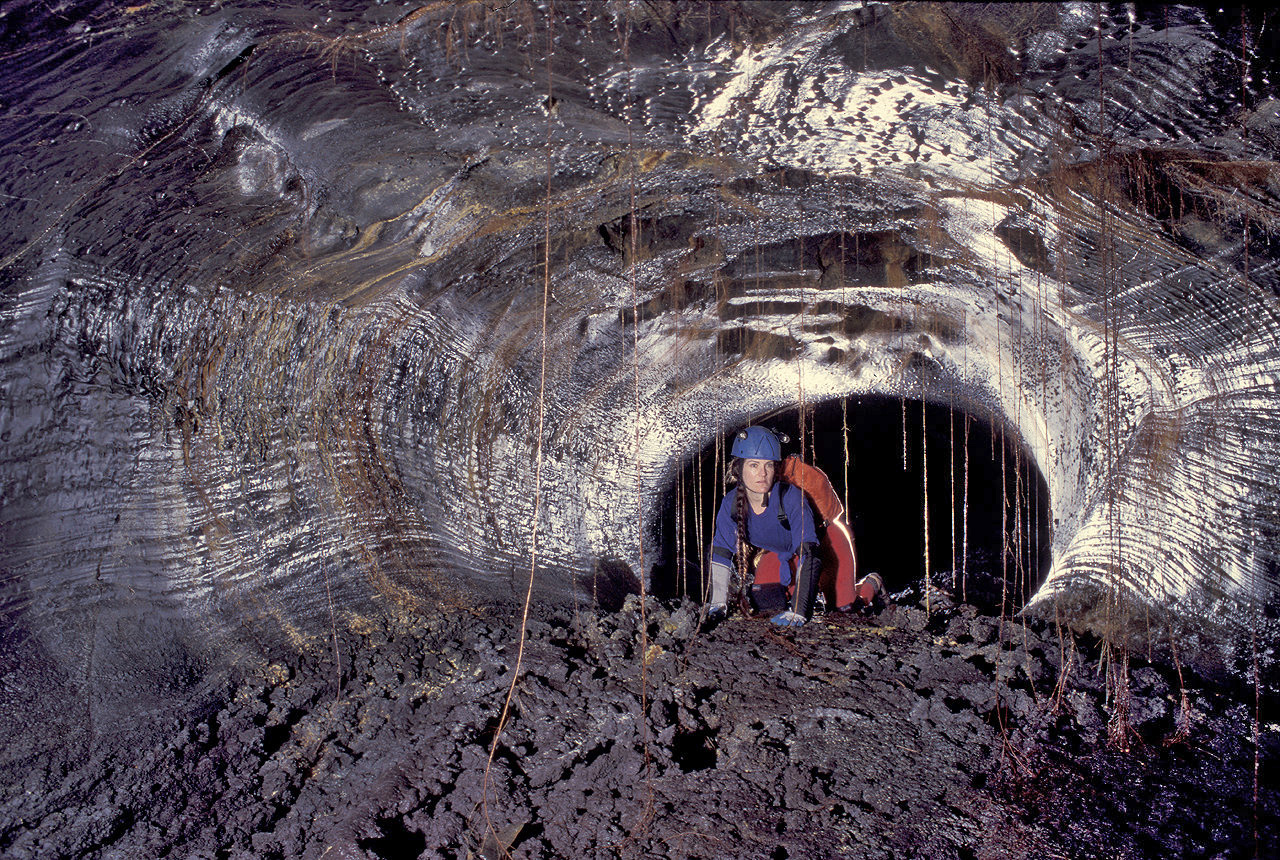
\includegraphics[height=1.5cm,width=1\textwidth,keepaspectratio]{surface_types/lava.jpg}
            \end{subfigure}
            \hfill
            \begin{subfigure}[b]{0.3\textwidth}
                \centering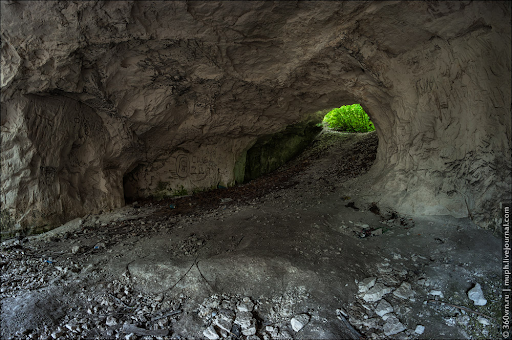
\includegraphics[height=1.5cm,width=1\textwidth,keepaspectratio]{surface_types/moul.png}
            \end{subfigure}
    
            \begin{subfigure}[b]{0.3\textwidth}
                \centering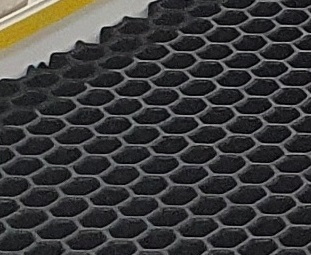
\includegraphics[height=1.5cm,width=1\textwidth,keepaspectratio]{surface_types/rubber.JPG}
            \end{subfigure}
            \hfill
            \begin{subfigure}[b]{0.3\textwidth}
                \centering\includegraphics[height=1.5cm,width=1\textwidth,keepaspectratio]{surface_types/rock.jpg}
            \end{subfigure}
            \hfill
            \begin{subfigure}[b]{0.3\textwidth}
                \centering\includegraphics[height=1.5cm,width=1\textwidth,keepaspectratio]{surface_types/zemlya.jpg}\\
            \end{subfigure}
            \vspace{-0.3cm}
            \caption{Эталоны упругой, твердой и пластичной поверхностей}
        \end{figure}
    \end{column}
\end{columns}
\end{frame}

\begin{frame}[t]{Стенд}
    \framesubtitle{}
    \begin{figure}[H]
        \begin{subfigure}{0.33\textwidth}
            \centering\includegraphics[height=4cm,width=1\textwidth,keepaspectratio]{s_shape_leg/rockk.png}
            \caption{Установка}
        \end{subfigure}
        \begin{subfigure}{0.33\textwidth}
            \centering\includegraphics[height=4cm,width=1\textwidth,keepaspectratio]{s_shape_leg/socks.jpg}
            \caption{Нога робота с установленными сенсорами}
        \end{subfigure}
        \begin{subfigure}{0.33\textwidth}
            \centering\includegraphics[height=4cm,width=1\textwidth,keepaspectratio]{s_shape_leg/leg_design.png}
            \caption{Схематическое распределение сенсоров на ноге}
        \end{subfigure}
    \end{figure}
\end{frame}

\begin{frame}[t]{Метод опорных векторов}
\framesubtitle{}
\small
\begin{columns}[T,onlytextwidth]
    \begin{column}{0.49\textwidth}
        \vspace{-0.5cm}
        \begin{align}
            f(x) = w^T x + b
        \end{align}
        где $x$ --- входной вектор, $w$ является весовым вектором, и $b$ --- смещение.

        Где \textbf{входной вектор}:

        (1) Частота движения ног\\
        (2-6) Пиковая и средняя амплитуда, среднее значение, ширина, площадь под кривой давления с датчика силы\\
        (7-11) Индивидуальная пиковая амплитуда силы для каждого датчика\\
        (12-15) Пиковая и средняя амплитуда, среднее значение, ширина, площадь под кривой  крутящего момента двигателя\\
        (16) Среднее давление на сенсорах
    \end{column}
    \begin{column}{0.49\textwidth}
        Ядро на основе функции Пирсона VII:
\begin{align}
    K(x, y) = (1 + ((||x - y||^2)/\sigma^2)^\omega)^{(-1/\omega)}
\end{align}
Где $x$, $y$ --- векторы во входном пространстве, $||x - y|||$ обозначает евклидово расстояние между $x$ и $y$, $\sigma$ --- масштабный параметр, определяющий <<разброс>> ядра, $\omega$ --- это параметр формы, который влияет на форму границы принятия решения.

\begin{figure}[H]
    \begin{subfigure}{0.49\textwidth}
        \centering\includegraphics[height=2cm,width=1\textwidth,keepaspectratio]{../images/s_shape_leg/avg_lin_vel_rev_min.png}
        \caption{График}
    \end{subfigure}
    \begin{subfigure}{0.49\textwidth}
        \centering\includegraphics[height=2cm,width=1\textwidth,keepaspectratio]{../images/s_shape_leg/TaxelIndForce.png}
        \caption{Таксель}
    \end{subfigure}
\end{figure}
    \end{column}
\end{columns}

    
\end{frame}

\begin{frame}[t]{Результаты}
    \framesubtitle{}
    \begin{figure}[H]
        \begin{subfigure}{0.49\textwidth}
            \caption{Таблица}
            \resizebox{\linewidth}{!}{%
                \begin{tabular}{|c|c|c|c|c|}
                    \cline{3-5}
                    \multicolumn{1}{l}{}                     & \multicolumn{1}{l|}{} & \multicolumn{3}{c|}{\textbf{Предсказанный класс}}                                                                                           \\
                    \cline{3-5}
                    \multicolumn{1}{l}{}                     &                       & Камень                                            & Резина                                     & Земля                                      \\
                    \hline
                    \multirow{3}{*}{{\textbf{Истин. класс}}} & Камень                & {\cellcolor[rgb]{0.741,0.843,0.929}}84.0\%        & 2.56\%                                     & 13.44\%                                    \\
                    \hhline{|~----|}
                                                             & Резина                & 20.1\%                                            & {\cellcolor[rgb]{0.741,0.843,0.929}}67.8\% & 12.1\%                                     \\
                    \hhline{|~----|}
                                                             & Земля                 & 1.0\%                                             & 18.9\%                                     & {\cellcolor[rgb]{0.741,0.843,0.929}}80.1\% \\
                    \hline
                \end{tabular}
            }
        \end{subfigure}
        \begin{subfigure}{0.49\textwidth}
            \centering\includegraphics[height=4cm,width=1\textwidth,keepaspectratio]{../images/s_shape_leg/feature_score.png}
            \caption{Feature score}
        \end{subfigure}
    \end{figure}
\end{frame}

\section{"1" Определение геометрических свойств поверхности}

\begin{frame}[t]{Определение геометрических свойств}
\framesubtitle{}
    \begin{columns}[T,onlytextwidth]
        \begin{column}{0.69\textwidth}
            \small
            Необходимо с помощью ощупывания роботом поверхности получить плотное облако точек и полигональную сетку.

            \textbf{Метод решения}: Триангуляция Делоне с использованием альфа формы

            \textbf{Идея решения}: Решив задачу локализации, получить облако точек следовой дорожки. Очистить шумное облако точек и его усреднить с помощью Voxel Grid, применить триангуляцию Делоне для вогнутых оболочек, получив полигональную сетку. Сгенерировать новые точки из полигональной сетки с нужным разрешением.

            \textbf{Входные данные}: следовая дорожка, в виде облака точек.
            
            \textbf{Выходные данные}: полигональная сетка и плотное облако точек
            
            \textbf{Допустимая точность}: 0.1 м, оценки Cloud2Cloud и Cloud2Mesh

            \textbf{Предположения}: 1) Имеется поверхность. Координаты задаются $z=f(x,y)$. 2) Расстояние между ногами робота мало относительно размеров поверхности, следовательно, поверхность между ногами считается плоскостью.   
        \end{column}
        \begin{column}{0.29\textwidth}
            \begin{figure}[H]
                \begin{subfigure}{0.99\textwidth}
                    \centering\includegraphics[height=2cm,width=1\textwidth,keepaspectratio]{../images/slides/delone_mag.png}
                    \caption{Пример Делоне}
                \end{subfigure}

                \begin{subfigure}{0.99\textwidth}
                    \centering\includegraphics[height=2cm,width=1\textwidth,keepaspectratio]{../images/slides/error.png}
                    \caption{Когда $z\neq f(x,y)$}
                \end{subfigure}
            \end{figure}
        \end{column}
    \end{columns}
\end{frame}

\begin{frame}[t]{Оценки C2C и C2M}
\framesubtitle{}
    \begin{figure}[H]
        \begin{subfigure}{0.49\textwidth}
            \centering\includegraphics[height=5cm,width=1\textwidth,keepaspectratio]{../images/slides/c2c.png}
            \caption{Cloud to Cloud}
        \end{subfigure}
        \begin{subfigure}{0.49\textwidth}
            \centering\includegraphics[height=5cm,width=1\textwidth,keepaspectratio]{../images/slides/c2m.png}
            \caption{Cloud to Mesh}
        \end{subfigure}
    \end{figure}
\end{frame}

\begin{frame}[t]{Эксперименты}
    \begin{figure}[H]
        \begin{subfigure}[t]{0.49\textwidth}
            \centering\includegraphics[height=5cm,width=1\textwidth,keepaspectratio]{coppelia_sim.png}
            \caption*{CoppeliaSim симулятор,\\ \textbf{4ое поколение} СтриРус}
        \end{subfigure}
        \begin{subfigure}[t]{0.49\textwidth}
            \centering\includegraphics[height=5cm,width=1\textwidth,keepaspectratio]{rl_sim.JPG}
            \caption*{Натурные испытания,\\ \textbf{3ье + поколение} СтриРус}
        \end{subfigure}
    \end{figure}
\end{frame}

\begin{frame}[t]{Задача локализации}
\framesubtitle{}
\begin{multline}
        H_{leg}^{glob} = H(x_{glob},y_{glob},z_{glob},\alpha_{glob},\beta_{glob},\gamma_{glob})T_z(l_1)T_x(l_2)R_y(\alpha_3)T_x(l_4)T_y(l_5)R_z(-15^{\circ})T_y(l_7)R_y(\alpha_8)
\end{multline}

\vspace{-0.3cm}
Где $H = \begin{bmatrix}
    \underset{3 \times 3}{R} & \underset{3 \times 1}{T} \\
    \underset{1 \times 3}{0} & \underset{1 \times 1}{1}
\end{bmatrix}$, $R_i$ --- матрица поворота, относительно одной из осей, $T_i$ --- вектор сдвига.

    \begin{columns}[T,onlytextwidth]
        \begin{column}{0.69\textwidth}
            
            \vspace{-0.3cm}
            \begin{figure}[H]
        \centering
        \begin{tikzpicture}
            % Include the image in a node
            \node [above right, inner sep=0] (image) at (0,0)
            {\centering\includegraphics[height=4.5cm,width=1\textwidth,keepaspectratio]{StriRus_10_legs_15_angle_v4.png}};
            % Create scope with normalized axes
            \begin{scope}[
                    x={($ 0.1*(image.south east)$)},
                    y={($ 0.1*(image.north west)$)}]
                % Grid and axes' labels
                % \draw[lightgray,step=1] (image.south west) grid (image.north east);
                % \foreach \x in {0,1,...,10} { \node [below] at (\x,0) {\x}; }
                % \foreach \y in {0,1,...,10} { \node [left] at (0,\y) {\y};}

                % Labels

                \coordinate (Xc) at (0.4415/2,-0.2347/2);
                \coordinate (Yc) at (-0.4512/2,-0.2156/2);
                \coordinate (Zc) at (0,0.5/2);
                % Labels
                \tikzstyle{origin} = [rounded corners=2pt, black, fill=gray!40, fill opacity=0.75, text opacity=1, scale=0.8,inner sep=1pt]
                \tikzstyle{transform_text} = [rounded corners=2pt, black, fill=white!85!gray, fill opacity=0.75, text opacity=1, scale=0.8,inner sep=1pt]
                \tikzstyle{transform_arrow} = [thick, green]

                % \coordinate (o_g) at (1,9);
                \node[circle,fill=green,scale=0.25] (o_g) at (1,9){};
                \draw[-stealth, very thick,blue] (o_g) -- ++(Xc);
                \draw[-stealth, very thick,green!70!black] (o_g) -- ++(Yc);
                \draw[-stealth, very thick,red] (o_g) -- ++(Zc);
                \node[origin,above right=3pt] at (o_g){\tiny $\mathbf{O_{glob}}$};

                % \coordinate (o_b) at (2.9,7.05);
                \node[circle,fill=green,scale=0.25] (o_b) at (2.9,7.05){};
                \draw[-stealth, very thick,blue] (o_b) -- ++(Xc);
                \draw[-stealth, very thick,green!70!black] (o_b) -- ++(Yc);
                \draw[-stealth, very thick,red] (o_b) -- ++(Zc);
                \node[origin,above right=2pt] at (o_b){\tiny $\mathbf{O_{base}}$};

                % \coordinate (o_1) at (2.9,6.6);
                \node[circle,fill=green,scale=0.25] (o_1) at (2.9,6.6){};
                \draw[-stealth, very thick,blue] (o_1) -- ++(Xc);
                \draw[-stealth, very thick,green!70!black] (o_1) -- ++(Yc);
                \draw[-stealth, very thick,red] (o_1) -- ++(Zc);
                \node[origin,above right=2pt] at (o_1){\tiny $\mathbf{O_{1}}$};

                % \coordinate (o_2) at (4,6);
                \node[circle,fill=green,scale=0.25] (o_2) at (4,6){};
                \draw[-stealth, very thick,blue] (o_2) -- ++(Xc);
                \draw[-stealth, very thick,green!70!black] (o_2) -- ++(Yc)
                node[origin,below=2pt]{\tiny $\mathbf{\alpha_3}$};
                \draw[-stealth, very thick,red] (o_2) -- ++(Zc);
                \node[origin,above right=2pt] at (o_2){\tiny $\mathbf{O_{2}=O_{3}}$};

                % \coordinate (o_4) at (7.0,4.55);
                \node[circle,fill=green,scale=0.25] (o_4) at (7.0,4.55){};
                \draw[-stealth, very thick,blue] (o_4) -- ++(Xc);
                \draw[-stealth, very thick,green!70!black] (o_4) -- ++(Yc);
                \draw[-stealth, very thick,red] (o_4) -- ++(Zc);
                \node[origin,above right=2pt] at (o_4){\tiny $\mathbf{O_{4}}$};

                % \coordinate (o_5) at (6.7,4.45);
                \node[circle,fill=green,scale=0.25] (o_5) at (6.7,4.45){};
                \draw[-stealth, very thick,blue] (o_5) -- ++(Xc);
                \draw[-stealth, very thick,green!70!black] (o_5) -- ++(Yc);
                \draw[-stealth, very thick,red] (o_5) -- ++(Zc);
                \node[origin,above left=3pt] at (o_5){\tiny $\mathbf{O_{5}=O_{6}}$};

                \coordinate (Xcr) at (0.49/2,0.07/2);
                % \coordinate (Ycr) at (-0.38/2,-0.32/2);
                \coordinate (Ycr) at (-0.24/2,-0.43/2);

                \draw[-stealth, very thick,blue] (o_5) -- ++(Xcr);
                \draw[-stealth, very thick,green!70!black] (o_5) -- ++(Ycr);


                % \coordinate (o_7) at (6.36,3.68);
                \node[circle,fill=green,scale=0.25] (o_7) at (6.36,3.68){};
                \draw[-stealth, very thick, blue] (o_7) -- ++(Xcr);
                \draw[-stealth, very thick, green!70!black] (o_7) -- ++(Ycr)
                node[origin,above left=2pt]{\tiny $\mathbf{\alpha_8}$};
                \draw[-stealth, very thick, red] (o_7) -- ++(Zc);
                \node[origin,below right=3pt] at (o_7){\tiny $\mathbf{O_{7}=O_{8}}$};

                \node[circle, draw ,fill=green,scale=0.4] (s_1) at (6.6,1.3){1};
                \node[circle,draw, fill=green,scale=0.4] (s_3) at (5.85,1.7){3};
                \node[circle,draw, fill=green,scale=0.4] (s_5) at (5.55,2.9){5};

                \draw[-stealth, transform_arrow] (o_g) -- (o_b)
                node[midway,below left=2pt, transform_text]{\tiny $\mathbf{H_{base}^{glob}}$};

                \draw[-stealth, transform_arrow] (o_b) -- (o_1)
                node[midway,left=3pt, transform_text]{\tiny $\mathbf{H_{1}^{base}}$};

                \draw[-stealth, transform_arrow] (o_1) -- (o_2)
                node[midway,below=2pt, transform_text]{\tiny $\mathbf{H_{2}^{1}}$};

                \draw[-stealth, transform_arrow] (o_2) -- (o_4)
                node[midway,below=2pt, transform_text]{\tiny $\mathbf{H_{4}^{3}}$};

                \draw[-stealth, transform_arrow] (o_4) -- (o_5)
                node[midway,below right=2pt, transform_text]{\tiny $\mathbf{H_{5}^{4}}$};

                \draw[-stealth, transform_arrow] (o_5) -- (o_7)
                node[midway,left=3pt, transform_text]{\tiny $\mathbf{H_{7}^{6}}$};

                \draw[-stealth, transform_arrow] (o_7) -- (s_1);
                \draw[-stealth, transform_arrow] (o_7) -- (s_3);
                \draw[-stealth, transform_arrow] (o_7) -- (s_5);
            \end{scope}
        \end{tikzpicture}
    \end{figure}
        \end{column}
        \begin{column}{0.29\textwidth}
            \begin{figure}[H]
                \centering\includegraphics[height=6cm,width=1\textwidth,keepaspectratio]{../images/slides/snow_local.png}
                \caption{Пример решения задачи локализации с помощью Aruco маркера}
            \end{figure}
        \end{column}
    \end{columns}
\end{frame}

\begin{frame}[t]{Делоне для вогнутых оболочек}
    \begin{figure}[H]
        \begin{subfigure}[t]{0.3\textwidth}
            \centering\includegraphics[height=5cm,width=1\textwidth,keepaspectratio]{convex_terr.png}
            \caption*{Пример поверхности}
            \label{fig:convex_terr.png}
        \end{subfigure}
        \hfill
        \begin{subfigure}[t]{0.33\textwidth}
            \centering
            \begin{tikzpicture}
                % Include the image in a node
                \node [above right, inner sep=0] (image) at (0,0)
                {\centering\includegraphics[height=6cm,width=1\textwidth,keepaspectratio]{conv_convex.png}};
                % Create scope with normalized axes
                \begin{scope}[
                        x={($ 0.1*(image.south east)$)},
                        y={($ 0.1*(image.north west)$)}]
                    % Grid and axes' labels
                    % \draw[lightgray,step=1] (image.south west) grid (image.north east);
                    % \foreach \x in {0,1,...,10} { \node [below] at (\x,0) {\x}; }
                    % \foreach \y in {0,1,...,10} { \node [left] at (0,\y) {\y};}

                    % Labels
                    \draw[stealth-, very thick,green] (5.2,3.5) -- ++(0,-1)
                    node[rounded corners=3pt,right,black,fill=white]{\tiny Полученная сетка};

                    \draw[stealth-, very thick,green] (5.5,5.5) -- (6.4,4)
                    node[rounded corners=3pt,right,black,fill=white]{\tiny Данные лидара};


                    \draw[stealth-, very thick,green] (3.4,0.8) -- (5,1);
                    \draw[stealth-, very thick,green] (3.4,2.6) -- (5,1)
                    node[rounded corners=3pt,right,black,fill=white]{\tiny Следовая дорожка};
                \end{scope}
            \end{tikzpicture}
            \caption*{Выпуклая оболочка}
            \label{fig:conv_convex.png}
        \end{subfigure}
        \hfill
        \begin{subfigure}[t]{0.33\textwidth}
            \centering\includegraphics[height=6cm,width=1\textwidth,keepaspectratio]{conv_concave.png}
            \caption*{Вогнутая оболочка}
            \label{fig:conv_concave.png}
        \end{subfigure}

    \end{figure}
\end{frame}

\begin{frame}[t]{Определение геометрических свойств поверхности}
    \framesubtitle{Результат: Маршрут, полигональная сетка}
    \vspace{-15pt}
    \begin{figure}[H]
        \begin{subfigure}[t]{0.36\textwidth}
            \centering\includegraphics[height=5cm,width=1\textwidth,keepaspectratio]{terrain_wo_water.png}
            \caption*{Начало маршрута}
        \end{subfigure}
        \begin{subfigure}[t]{0.36\textwidth}
            \centering\includegraphics[height=5cm,width=1\textwidth,keepaspectratio]{terrain_w_water_end.png}
            \caption*{Конец маршрута}
        \end{subfigure}
        \begin{subfigure}[t]{0.26\textwidth}
            \centering\includegraphics[height=5cm,width=1\textwidth,keepaspectratio]{mesh_rviz.png}
            \caption*{Созданная сетка}
        \end{subfigure}
    \end{figure}


\end{frame}

\begin{frame}[t]{Определение геометрических свойств поверхности}
    \framesubtitle{Результаты Cloud2Cloud и Cloud2Mesh}
    \vspace{-15pt}
    \begin{figure}[H]
        \begin{subfigure}[t]{0.49\textwidth}
            \centering
            \begin{tikzpicture}
                % Include the image in a node
                \node [above right, inner sep=0] (image) at (0,0)
                {\centering\includegraphics[height=2.8cm,width=1\textwidth,keepaspectratio]{sampled_pcd.png}};
                % Create scope with normalized axes
                \begin{scope}[
                        x={($ 0.1*(image.south east)$)},
                        y={($ 0.1*(image.north west)$)}]
                    % Grid and axes' labels
                    % \draw[lightgray,step=1] (image.south west) grid (image.north east);
                    % \foreach \x in {0,1,...,10} { \node [below] at (\x,0) {\x}; }
                    % \foreach \y in {0,1,...,10} { \node [left] at (0,\y) {\y};}

                    % Labels
                    \draw[stealth-, very thick,green] (3,8) -- (2,8.5);
                    \draw[stealth-, very thick,green] (1,5.5) -- (2,8.5)
                    node[rounded corners=3pt,above,black,fill=white]{\tiny Эталонное Облако};

                    \draw[stealth-, very thick,green] (5.5,3) -- (5.5,8.5)
                    node[rounded corners=3pt,above,black,fill=white]{\tiny Сгенерированное Облако};
                \end{scope}
            \end{tikzpicture}
            % \caption*{Наложенные облака точек}
            \label{fig:sampled_pcd.png}
        \end{subfigure}
        \begin{subfigure}[t]{0.49\textwidth}
            \centering\includegraphics[height=2.8cm,width=1\textwidth,keepaspectratio]{mesh_comp.png}
            % \caption*{Наложенные сетки}
        \end{subfigure}

        \begin{subfigure}[t]{0.49\textwidth}
            \centering\includegraphics[height=2.6cm,width=1\textwidth,keepaspectratio]{pcd_hist.png}
            \caption*{Гистограмма ошибок C2C}
        \end{subfigure}
        \begin{subfigure}[t]{0.49\textwidth}
            \centering\includegraphics[height=2.6cm,width=1\textwidth,keepaspectratio]{mesh_hist.png}
            \caption*{Гистограмма ошибок C2M}
        \end{subfigure}
    \end{figure}
\end{frame}

\begin{frame}[t]{Определение геометрических свойств поверхности}
    \framesubtitle{Результат: Натурные испытания, Видео}
    \vspace{-0.5cm}
    \begin{figure}[H]
        \begin{subfigure}[t]{0.49\textwidth}
            % \href{run:./videos/big_angle2.mp4}{
            \href{https://youtu.be/2dxHHTG4psQ}{
                \centering\includegraphics[height=6cm,width=1\textwidth,keepaspectratio]{real_robot_mesh_video_preview.png}}
            \caption*{Робот проходит препятствие}
        \end{subfigure}
        \begin{subfigure}[t]{0.49\textwidth}
            \centering\includegraphics[height=6cm,width=1\textwidth,keepaspectratio]{real_mesh.jpg}
            \caption*{Полигональная сетка, полученная с помощью ног}
        \end{subfigure}
    \end{figure}
\end{frame}

\section{Выводы}

\begin{frame}[t]{Результаты решения задач}
    \framesubtitle{}
    \begin{columns}[T,onlytextwidth]
        \begin{column}{0.48\textwidth}
            \begin{block}{Научных задач (научная новизна)}
                1. Метод \textbf{подбора количества ног для шагающих цикловых движителей}.

                2. Методика \textbf{характеризации датчика}, когда площадь касания нагрузки меньше, чем размеры датчика.

                3. Алгоритмы \textbf{калибровки} и \textbf{определения физических свойств поверхности}.

                4. Метод определения \textbf{геометрических свойств местности}.

            \end{block}
        \end{column}
        \begin{column}{0.48\textwidth}
            \begin{alertblock}{Экспериментальных разработок}
                1. Спроектированы и собраны 2 прототипа с \textbf{Шагающим цикловым движителем} с одной степенью свободы в ноге.

                2. Разработана и создана \textbf{экспериментальная установка} для \textbf{автоматизированного исследования датчика силы}.

                3. Разработана и создана \textbf{экспериментальная установка} для \textbf{определения типа поверхности}.

            \end{alertblock}
        \end{column}
    \end{columns}
\end{frame}

\begin{frame}[t]{Результаты интеллектуальной деятельности}
    \framesubtitle{}
    \begin{itemize}
        \item \textit{Количество публикаций}
              \begin{itemize}
                  \large
                  \item \textbf{2} --- журналы, рекомендованных ВАК
                  \item \textbf{3} --- журналы, индексируемые в Scopus (2 работы Q2)
                  \item \textbf{5} --- РИНЦ
              \end{itemize}
        \item \textbf{8} --- Зарегистрированных программ для ЭВМ
        \item \textbf{3} --- Выигранных гранта (Умник, ЦНТИ, РФФИ)
    \end{itemize}
\end{frame}



\begin{frame}[t]{Соответствие паспорту специальности}
    \framesubtitle{2.5.4 Робототехника, Роботы, мехатроника и
    робототехнические системы}
    1. Развитие теоретических основ и методов анализа, структурного и параметрического синтеза и автоматизированного проектирования роботов и робототехнических систем. \\
    7. Методы экспериментального исследования, создания прототипов и
    экспериментальных стендов и модульных платформ для разработки роботов, робототехнических и мехатронных систем. \\
    9. Методы расчета и проектирования мехатронных сервоприводов,
    исполнительных, сенсорных и управляющих компонентов роботов,
    робототехнических и мехатронных систем.
\end{frame}

% \begin{frame}[t]{Апробация работы}
%     \framesubtitle{Статьи в периодических изданиях по перечню ВАК РФ}
%     \begin{enumerate}
%         \item Буличев О. В., Полёткин К. В., Малолетов А. В. Исследование характеристик датчика силы на основе материала «Velostat» для мобильного шагающего робота // Известия Волгоградского государственного технического университета. 2022. № 4. C. 6–12.
%         \item Буличев О. В., Малолетов А. В. Метод оптимизации количества ног шагающего робота на основе эволюционного алгоритма // Известия Волгоградского государственного технического университета. 2022. № 9. C. 12–19.
%     \end{enumerate}
% \end{frame}

\fbckg{fibeamer/figs/last_page.png}
\frame[plain]{}
\fbckg{fibeamer/figs/common.png}

\end{document}